% !TeX root = ../main.tex

\chapter{理论}
\label{cha:Theory}

粒子物理是物理学的一个分支,是研究组成物质世界的
%不可分割的最小可检测的
最基本的粒子和它们之间相互作用的一门学科,
目前解释已知的基本粒子和它们之间相互作用的动力学的
%主要的也是
最成功的理论是标准模型(The Standard Model, SM)
~\cite{SM1,SM2,SM3,SM4,SM5,SM6,SM7,SMTALK,SM8,SMBOOK}。
从1897年J.J.Thomson首次在实验中发现电子~\cite{THOMSON},到2012年标准模型中最后一个粒子希格斯玻色子的发现~\cite{ATLASHIGGS,CMSHIGGS},
标准模型经过一百多年的发展逐渐完善,其不仅理论上自洽,而且在实验预测上也非常的成功。
尽管如此,物理学家在
%理论和实验研究中
试图将其扩展成为一个包含所有常数和物理现象的“终极理论”的时候,
发现仍有一些不足之处亟待解决,比如标准模型没有解释暗物质~\cite{DARKMATTER1,DARKMATTER2}从何而来、没有包含引力子~\cite{GRAVITON}、
也没有解释宇宙中正反物质不对称~\cite{ANTIMATTER}和中微子质量起源~\cite{NEUTRINO1,NEUTRINO2}等问题。

本章第~\ref{sec:SM}~小节将简要介绍标准模型,包括各种相互作用、对称性自发破缺和希格斯玻色子,
接着在第~\ref{sec:Higgs}~小节会介绍希格斯玻色子的性质和高横动量希格斯玻色子衰变到双b夸克的标定动机,
最后第~\ref{sec:BSM}~小节简要介绍在双喷注末态的不变质量谱中寻找超出标准模型的新物理的动机和所用到的基准新物理模型。

\section{标准模型}
\label{sec:SM}


由于覆盖范围广、预测能力强以及对已知的基本粒子之间相互作用的精确描述,
粒子物理中的标准模型被认为是现有最全面而且最强大的物理理论之一。
它的目标是对亚原子粒子进行分类,并准确描述它们之间的相互作用和自相互作用,
类似于元素周期表,标准模型可以根据其属性对所有已知的基本粒子进行排布。
量子场论(Quantum Field Theory, QFT)~\cite{QFT1}是严格描述和构建标准模型的数学基础,
它协调了量子力学~\cite{QMP}和狭义相对论~\cite{SRE},
在这个基础之上,粒子被视为相应场的量子化激发,
而场是将标量、矢量或张量与时空中每个点关联起来的函数,
相互作用可以通过各种场的理论来描述。
标准模型的构建遵循对称性原则,而拉格朗日量是描述物理系统动力学的基本手段,又称拉氏量,
因此物理体系的基本对称性是通过体系拉氏量的对称性来体现的。
与理论相联系的实验观测量比如散射截面和衰变宽度等可以利用
微扰论的方法得到~\cite{QFT1}。

\subsection{最小作用量原理}
\label{sec:LAP}
类似于经典力学,物理系统的动力学特征可以由最小作用量原理~\cite{ACTION1,ACTION2}得到,
首先,定义一个体系的作用量S:
\begin{equation} 
\label{eq:ACTION1}
S=\int d^4x \quad \mathcal{L}\left[ \phi_i(x),\partial_{\mu}\phi_i(x) \right]
\end{equation}
其中四维时空的积分$\int d^4x$保持洛伦兹不变性,
体系的拉氏量密度$\mathcal{L}$是场$\phi_i(x)$和它们的偏导$\partial_{\mu}\phi_i(x)$的函数,
它也具有洛伦兹不变性。
最小作用量原理要求作用量的变化$\delta S$在场的微小变化$\delta \phi_i$之下为零,
假设$\delta \phi_i$是可微的并且在时空的某个有界区域之外为零,
由$\delta S=0$可以得到场的欧拉-拉格朗日运动方程:
\begin{equation} 
\label{eq:ACTION2}
\frac{\partial\mathcal{L}}{\partial\phi_i}-\partial^{\mu}\left( \frac{\mathcal{L}}{\partial(\partial^{\mu}\phi_i)} \right) =0
\end{equation}

\subsection{对称性和守恒律}
\label{sec:SCL}
假设在一组连续的变换下:
\begin{equation} 
\label{eq:ACTION3}
\phi_i(x) \rightarrow \phi'_i(x)=\phi_i(x)+\epsilon\delta_{\epsilon}\phi_i(x)+O(\epsilon^2)
\end{equation}
体系的拉氏量保持不变:
\begin{equation} 
\label{eq:ACTION4}
\mathcal{L}\left[ \phi_i(x),\partial_{\mu}\phi_i(x) \right]=\mathcal{L}\left[ \phi'_i(x),\partial_{\mu}\phi'_i(x) \right]
\end{equation}
那么可以得到:
\begin{equation} 
\label{eq:ACTION5}
\delta_{\epsilon}\mathcal{L} \quad = \quad 0 \quad = \quad \sum_i \Bigg\{ \left[ \frac{\partial\mathcal{L}}{\partial\phi_i}-\partial^{\mu}\left( \frac{\partial\mathcal{L}}{\partial(\partial^{\mu}\phi_i)} \right) \right] \delta_{\epsilon}\phi_i + \partial^{\mu}  \left[  \frac{\partial\mathcal{L}}{\partial(\partial^{\mu}\phi_i)}\delta_{\epsilon}\phi_i  \right]   \Bigg\}
\end{equation}
上式右边第一项便是欧拉-拉格朗日运动方程~\ref{eq:ACTION2}~,其值为零,
化简之后,体系有一个守恒流:
\begin{equation} 
\label{eq:ACTION6}
J_{\mu}\equiv\sum_i \frac{\mathcal{L}}{\partial(\partial^{\mu}\phi_i)}\delta_{\epsilon}\phi_i , \quad \partial^{\mu}J_{\mu}=0
\end{equation}
其中第一项定义为守恒荷:
\begin{equation} 
\label{eq:ACTION7}
Q \equiv \int d^3x J^0
\end{equation}
式~\ref{eq:ACTION6}~中的条件$\partial^{\mu}J_{\mu}=0$保证了$\frac{dQ}{dt}=0$,因此Q是个守恒量。
这种关系被称为Noether定理~\cite{NOETHER},
%可以将其扩展到
在涉及时空坐标的一般变换中,
对于每一个使作用量保持不变的连续对称变换,
都会出现一个相应的守恒流,因此也会有一个守恒荷。

标准模型包含了三种基本的相互作用:强相互作用、弱相互作用和电磁相互作用。
这三种基本相互作用的构建是基于三种不同的对称性,
与基本的相互作用关联的这些对称性被称为局部规范对称性,
对称性的数学基础是群论~\cite{GROUP},
从而,标准模型是通过三个代表对称性的群$SU(3)	\otimes SU(2)	\otimes U(1)$构建起来的:
%对称群$SU(3)$反应的是强相互作用的对称性,
强相互作用的对称性群是$SU(3)$,由量子色动力学描述,
与这个对称性相对应的守恒荷为色荷;
%对称群$SU(2)	\otimes U(1)$反应的是电磁和弱相互作用的对称性
电磁和弱相互作用的对称性群$SU(2)	\otimes U(1)$,用电弱理论描述;
电磁相互作用的对称性群为$U(1)$,由量子电动力学描述,
与这个对称性相对应的守恒荷为电荷。

%$U(1)$可以单独描述电磁相互作用的对称性,相应的理论为量子电动力学,守恒荷为电荷。
另外,由狭义相对论的要求,标准模型需满足最基本的洛伦兹对称性,这种对称性是全局对称性,
相应的对称性群为洛伦兹群,由于洛伦兹群特殊的拓扑性质,
标准模型对基本粒子分类时需引入一个被称为自旋的内禀属性~\cite{QFT1},它只能取整数或者半整数,
自旋为半整数的粒子被称为费米子,自旋为整数的粒子被称为玻色子。
标准模型中的质量也是粒子的一个内禀属性,
它是由粒子所对应的场与希格斯玻色子所对应的场的耦合引起的,
其中希格斯玻色子是标准模型中唯一一个自旋为0的基本粒子,后文将会介绍。
这里引入这些基本属性是为了在下一小节对基本粒子进行分类。

\subsection{基本粒子}
\label{sec:EP}

标准模型中基本粒子没有内部结构,不可再分。
如图~\ref{fig:SM1}~所示,它们可以分为自旋为$\frac{1}{2}$的费米子、自旋为1的规范玻色子和自旋为0的标量玻色子希格斯玻色子三部分。
费米子遵循费米-狄拉克统计~\cite{FERMIS1,FERMIS2},又可以分为夸克(q)和轻子两部分,其中轻子按其质量和相互作用特点可以分为三代:
\begin{equation} 
\label{eq:EP1}
\left( \begin{aligned}
e^-\\ \nu_e
\end{aligned}
\right)
\quad
\left( \begin{aligned}
\mu^-\\ \nu_{\mu}
\end{aligned}
\right)
\quad
\left( \begin{aligned}
\tau^-\\ \nu_{\tau}
\end{aligned}
\right)
\end{equation}
轻子可以参与电磁和弱相互作用,它们之中的$(e^-,\mu^-,\tau^-)$既能参与电磁相互作用又能参与弱相互作用,
因此带有电荷,且所带电荷量相等都为-e,它们的质量都不为0并依次递增;
$(\nu_e,\nu_{\mu},\nu_{\tau})$被称为中微子,与三个轻子有一一对应的关系,它们仅参与弱相互作用,无质量,
但是实验上观测到了中微子振荡的现象,表明中微子质量并不为0~\cite{NEUTRINO1,NEUTRINO2}。

夸克按其质量递增和作用特点也分为三代共6个:
\begin{equation} 
\label{eq:EP2}
\left( \begin{aligned}
u\\ d
\end{aligned}
\right)
\quad
\left( \begin{aligned}
c\\ s
\end{aligned}
\right)
\quad
\left( \begin{aligned}
t\\ b
\end{aligned}
\right)
\end{equation}
它们能同时参与电磁、弱和强相互作用,因此它们都带有电荷和色荷,
其中$(u,c,t)$所带电荷量为$\frac{2}{3}e$,$(d,s,b)$所带电荷量为$-\frac{1}{3}e$,
色荷共有三种
%$(red,green,blue)$
,它们能带其中的任意一种。

玻色子遵从玻色-爱因斯坦统计~\cite{BOSON},
规范玻色子共$(g,\gamma,Z,W)$四种,它们用于传递费米子之间的基本相互作用:
光子$\gamma$是无质量粒子,用于传递带电荷粒子之间的电磁相互作用;
W和Z玻色子质量比较大,可以传递
%中微子参与的
弱相互作用;
胶子g是强相互作用的媒介子,无质量。
标量玻色子希格斯玻色子不带电荷,质量大约在125GeV,
%希格斯玻色子$H$是标准模型中唯一一个自旋为0的标量玻色子,
它与标准模型中其他基本粒子的质量起源有关,在第~\ref{sec:SSB}~小节将会介绍。
另外,根据CPT定理~\cite{CPT1,CPT2},每个粒子都会有一个与之对应的反粒子,
它们之间质量和自旋都相等,所带电荷和色荷相反。

\begin{figure}
  \begin{center}
    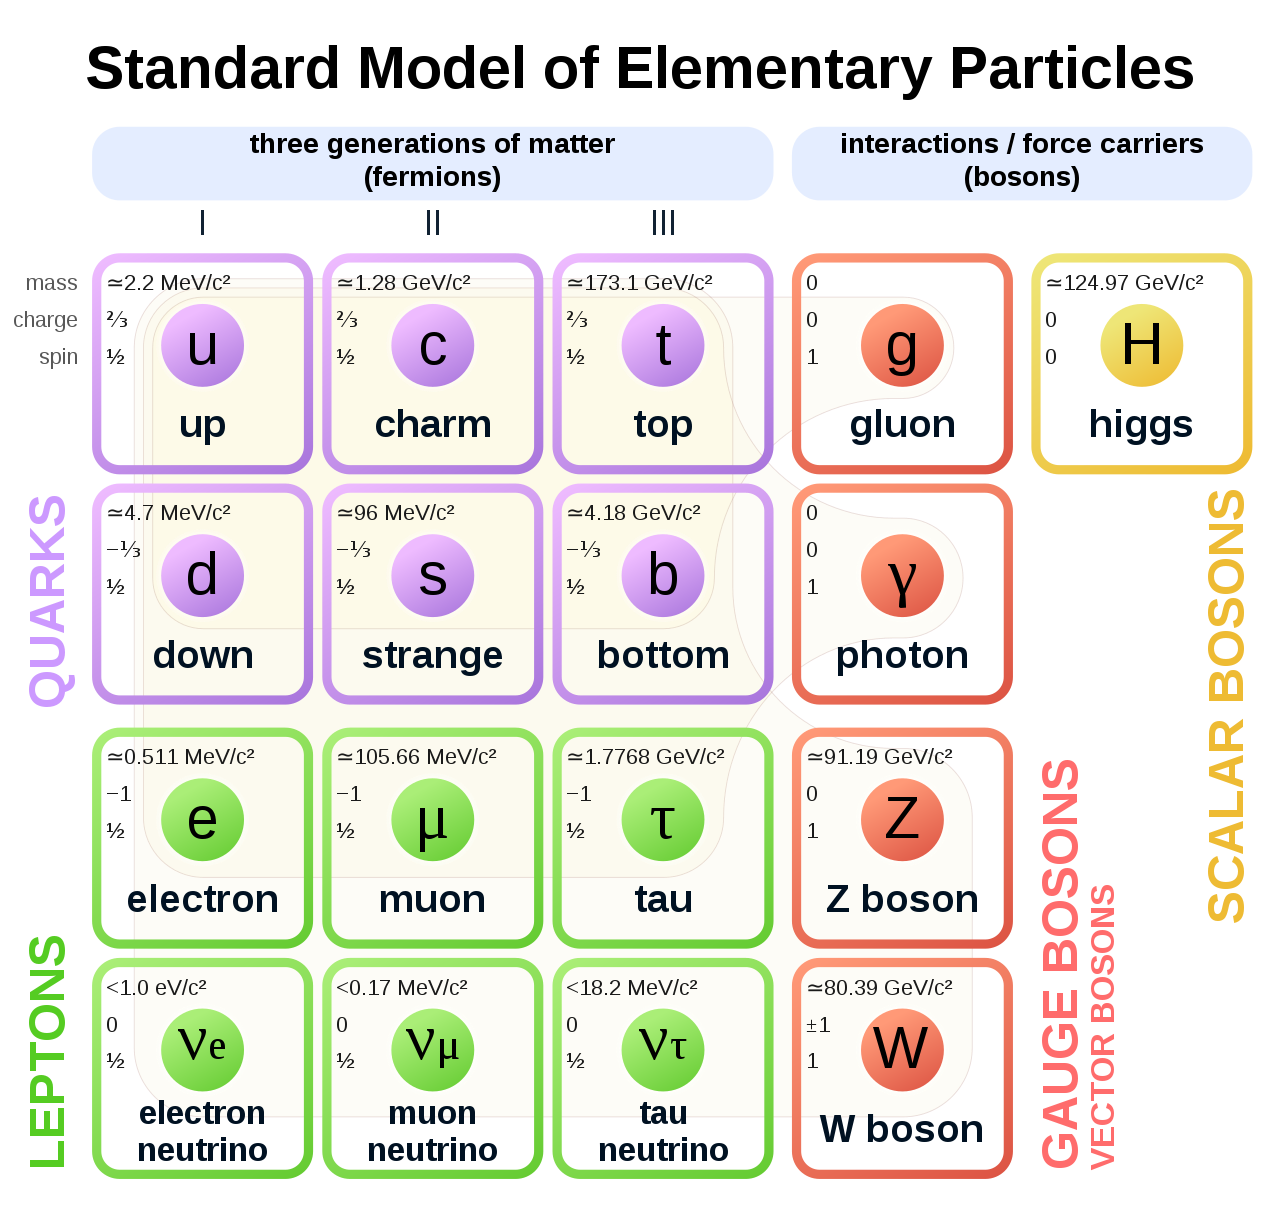
\includegraphics[width=0.75\textwidth]{figuresTHE/SM1.png}
  \end{center}
  \caption{ 标准模型中的基本粒子。图中还显示了各个粒子的质量、电荷和自旋。}
    \label{fig:SM1}
\end{figure}

\subsection{量子电动力学}
\label{sec:QED}
量子电动力学(Quantum electrodynamics, QED)是量子场论中最为成功的理论之一,
它描述了带电粒子之间的电磁相互作用,是一个阿贝尔规范理论~\cite{GAUGE1},
建立在对称群$U(1)$之上,规范场即为电磁场。
对于一个自由的狄拉克费米子$\psi(x)$,其拉氏量$\mathcal{L}_0$为:
\begin{equation} 
\label{eq:QED1}
\mathcal{L}_0= i \bar{\psi}(x) \gamma^{\mu} \partial_{\mu} \psi(x) - m \bar{\psi}(x) \psi(x)
\end{equation}
它在全局$U(1)$对称变换下是不变的:
\begin{equation} 
\label{eq:QED2}
\psi(x) \rightarrow (\psi(x))' = exp\{  i\theta \} \psi(x)
\end{equation}
其中$exp\{  i\theta \} \psi(x)$是$U(1)$的表示,$\theta$为任意实数常数,当重新定义这个变换使它依赖于时空坐标$\theta=\theta(x)$,即局部$U(1)$规范变换,
则破坏了拉氏量$\mathcal{L}_0$的不变性:
\begin{equation} 
\label{eq:QED3}
\partial_{\mu} \psi(x)  \rightarrow exp\{  i\theta(x) \} (\partial_{\mu} + i\partial_{\mu}\theta(x) ) \psi(x)
\end{equation}
规范原理要求拉氏量$\mathcal{L}_0$此时仍然保持不变性,
则需要引入一个自旋为1的矢量场$A_{\mu}(x)$,即电磁场,来抵消上述第二项,它服从变换:
\begin{equation} 
\label{eq:QED4}
A_{\mu}(x) \rightarrow A'_{\mu}(x) = A_{\mu}(x)- \frac{1}{e} \partial_{\mu}\theta(x)
\end{equation}
其中e是耦合常数,由此在偏微分基础上定义协变微分$D_{\mu}$:
\begin{equation} 
\label{eq:QED5}
D_{\mu}\psi(x) \equiv \left[ \partial_{\mu}+ieA_{\mu}(x) \right] \psi(x)
\end{equation}
它的变换可以与费米场的变换相互抵消:
\begin{equation} 
\label{eq:QED6}
D_{\mu}\psi(x) \rightarrow (D_{\mu}\psi)'(x)= exp\{  i\theta(x) \} D_{\mu}\psi(x)
\end{equation}
另外矢量场$A_{\mu}(x)$的自由拉氏量$\mathcal{L}_1$是:
\begin{equation} 
\label{eq:QED7}
\mathcal{L}_1=-\frac{1}{4}F_{\mu\nu}(x)F^{\mu\nu}(x)
\end{equation}
结合上述,可以得到最终的QED拉氏量$\mathcal{L}_{QED}$:
%\begin{equation} 
%\label{eq:QED8}
 %\begin{aligned}
 % \mathcal{L}_{QED} = i \bar{\psi}(x) \gamma^{\mu} D_{\mu} \psi(x) - m \bar{\psi}(x) \psi(x) + \mathcal{L}_1
  %\\
 % = i \bar{\psi}(x) \gamma^{\mu} \partial_{\mu} \psi(x) - m \bar{\psi}(x) \psi(x) - e A_{\mu}(x) 
  %\bar{\psi}(x) \gamma^{\mu} \psi(x) - -\frac{1}{4}F_{\mu\nu}(x)F^{\mu\nu}(x)
 %\end{aligned}
%\end{equation}
\begin{equation}
\label{eq:QED8}
\begin{split}
\mathcal{L}_{QED} & =i \bar{\psi}(x) \gamma^{\mu} D_{\mu} \psi(x) - m \bar{\psi}(x) \psi(x) + \mathcal{L}_1\\
& = i \bar{\psi}(x) \gamma^{\mu} \partial_{\mu} \psi(x) - m \bar{\psi}(x) \psi(x) \\
&\quad - e A_{\mu}(x)\bar{\psi}(x) \gamma^{\mu} \psi(x) - -\frac{1}{4}F_{\mu\nu}(x)F^{\mu\nu}(x)
\end{split}
\end{equation}
它在局部$U(1)$规范变换下保持不变,
其中第一项和第二项是狄拉克费米子场的自由拉氏量;
%将在后续介绍希格斯玻色子之后重新给出;
第三项是带电费米子与电磁场的电磁相互作用项;
第四项是电磁场的动能项,
由于电磁场的质量项$\frac{1}{2}m^2A^{\mu}A_{\mu}$在局部规范变换下不具有不变性,
因此光子没有质量。



\subsection{量子色动力学}
\label{sec:QCD}
量子色动力学(Quantum chromodynamics, QCD)是描述由胶子g作为媒介子的夸克之间强相互作用的理论,
它是一个非阿贝尔规范理论~\cite{SM0},建立在局部规范对称群$SU(3)$的基础上。
对于夸克场$q_f^{\alpha}$,其中$\alpha$是色荷指标,$f$为夸克的味指标,体系自由拉氏量$\mathcal{L}_0$为:
\begin{equation} 
\label{eq:QCD1}
\mathcal{L}_0=\sum_f \bar{q}_f (i\gamma^{\mu}\partial_{\mu}-m_f)q_f
\end{equation}
其在色荷空间中任意的全局对称变换$SU(3)$下是不变的:
\begin{equation} 
\label{eq:QCD2}
 \begin{split}
 &  q_f^{\alpha} \rightarrow (q_f^{\alpha})'=U^{\alpha}_{~\beta}q_f^{\beta}  \\
 & UU^{\dagger} =U^{\dagger}U=1, \quad det~U=1
 \end{split}
\end{equation}
其中$U$是$SU(3)$的矩阵表示,可以写成如下形式:
\begin{equation} 
\label{eq:QCD3}
U=exp\Bigg\{ i\frac{\lambda^{a}}{2}\theta_a \Bigg\} 
\end{equation}
这里$\frac{\lambda^{a}}{2}(a=1,2,\dots,8)$是李代数$SU(3)$基础表示中的八个生成元,$\theta_a$是任意参数。
生成元$\frac{\lambda^{a}}{2}$之间满足如下代数关系:
\begin{equation} 
\label{eq:QCD4}
\left[ \frac{\lambda^{a}}{2}, \frac{\lambda^{b}}{2} \right]=if^{abc}\frac{\lambda^{c}}{2}
\end{equation}
其中$f^{abc}$是李代数$SU(3)$的结构参数。

类似量子电动力学,当要求自由拉氏量$\mathcal{L}_0$在$SU(3)$局部规范变换下保持不变:
\begin{equation} 
\label{eq:QCD5}
U(x)=exp\Bigg\{ i\frac{\lambda^{a}}{2}\theta_a(x) \Bigg\} 
\end{equation}
由于$U(x)$包含八个独立的规范参数,需要将偏微分$\partial_{\mu}$换成协变微分$D_{\mu}$并引入八个独立的规范场以保证拉氏量$\mathcal{L}_0$的不变性:
\begin{equation} 
\label{eq:QCD6}
D^{\mu}q_f=\left[   \partial^{\mu}+ig_s\frac{\lambda^{a}}{2}G^{\mu}_a(x)  \right] q_f \equiv
\left[   \partial^{\mu}+ig_sG^{\mu}(x) \right] q_f
\end{equation}
其中$g_s$为耦合常数,八个规范场$G^{\mu}_a(x)$即对应于八个不同的规范玻色子,胶子。
这里引入了一个缩写表示:
\begin{equation} 
\label{eq:QCD7}
\left[G^{\mu}(x)\right]_{\alpha\beta} \equiv \left( \frac{\lambda^{a}}{2} \right)_{\alpha\beta}G^{\mu}_a(x) 
\end{equation}
当要求协变微分项$D^{\mu} q_f$与色荷矢量$q_f$以完全相同的方式进行变换,可以得到规范场$G^{\mu}$的变换属性:
\begin{equation} 
\label{eq:QCD8}
D^{\mu} \rightarrow (D^{\mu})' = UD^{\mu}U^{\dagger}, \quad 
G^{\mu} \rightarrow (G^{\mu})'=UG^{\mu}U^{\dagger}+\frac{i}{g_s}(\partial^{\mu}U)U^{\dagger}
\end{equation}
由此,在$SU(3)$局部规范变换下有:
\begin{equation} 
\label{eq:QCD9}
 \begin{split}
  & q_f^{\alpha}\rightarrow (q_f^{\alpha})'=q_f^{\alpha}+i\left( \frac{\lambda^{a}}{2} \right)_{\alpha\beta}\delta\theta_a q_f^{\beta}
   \\
  & G^{\mu}_a\rightarrow (G^{\mu}_a)'=G^{\mu}_a-\frac{1}{g_s}\partial^{\mu}\left(\delta\theta_a\right)-f^{abc}\delta\theta_bG^{\mu}_c
  \end{split}
\end{equation}
由于李代数$SU(3)$的非交换性,使得QCD中规范场的规范变换比QED中规范场光子的变换要复杂很多,
拉氏量中会出现了涉及胶子场自身的附加项,
并且带有不同色荷的夸克都以完全相同的耦合强度$g_s$与胶子场耦合。

为了构建胶子场的动力学,引入相应的场强$G^{\mu\nu}(x)$:
\begin{equation} 
\label{eq:QCD10}
 \begin{split}
  & G^{\mu\nu}(x) \equiv -\frac{i}{g_s}\left[D^{\mu},D^{\nu} \right] = \partial^{\mu}G^{\nu}-\partial^{\nu}G^{\mu} +i g_s\left[G^{\mu},G^{\nu} \right]
   \equiv \frac{\lambda^{a}}{2}G^{\mu\nu}_a(x)
   \\
&   G^{\mu\nu}_a(x)= \partial^{\mu}G^{\nu}_a-\partial^{\nu}G^{\mu}_a -g_sf^{abc}G^{\mu}_bG^{\nu}_c 
 \end{split}
\end{equation}
在$SU(3)$规范变化下有:
\begin{equation} 
\label{eq:QCD11}
G^{\mu\nu} \rightarrow  (G^{\mu\nu})'=UG^{\mu\nu}U^{\dagger}
\end{equation}
并且$\frac{1}{2}G^{\mu\nu}_a G^a_{\mu\nu}=Tr(G^{\mu\nu}G_{\mu\nu})$是不变的,
最终可以得到完整的$SU(3)$局部规范不变的QCD拉氏量:
\begin{equation} 
\label{eq:QCD12}
\mathcal{L}_{QCD}  \equiv  -\frac{1}{4}G^{\mu\nu}_a G_{\mu\nu}^a +\sum_f \bar{q}_f (i\gamma^{\mu}D_{\mu}-m_f)q_f
\end{equation}
由式~\ref{eq:QCD8}~可知胶子场的质量项$\frac{1}{2}m^2_G G^{\mu}_a G^a_{\mu}$在$SU(3)$规范变换下不是不变的,
因此它不会出现在拉氏量$\mathcal{L}_{QCD}$中,
这表明胶子是无质量的规范玻色子。

将拉氏量$\mathcal{L}_{QCD}$展开之后:
\begin{equation} 
\label{eq:QCD13}
 \begin{split}
   \mathcal{L}_{QCD}  \quad = \quad & -\frac{1}{4} (\partial^{\mu}G^{\nu}_a-\partial^{\nu}G^{\mu}_a) (\partial_{\mu}G_{\nu}^a-\partial_{\nu}G_{\mu}^a)+
   \sum_f \bar{q}^{\alpha}_f (i\gamma^{\mu}\partial_{\mu}-m_f)q^{\alpha}_f
   \\
  & -g_s G^{\mu}_a \sum_f \bar{q}^{\alpha}_f \gamma^{\mu} \left( \frac{\lambda^{a}}{2} \right)_{\alpha\beta} q^{\beta}_f
   \\
  & +\frac{g_s}{2} f^{abc} (\partial^{\mu}G^{\nu}_a-\partial^{\nu}G^{\mu}_a) G^b_{\mu} G^c_{\nu} 
   -\frac{g_s^2}{4} f^{abc} f_{ade} G_b^{\mu} G_c^{\nu}  G^d_{\mu} G^e_{\nu} 
 \end{split}
\end{equation}
其中第一行第一项是胶子的动能项,
第二项是夸克场的自由拉氏量;
%,将在后续介绍希格斯玻色子之后重新给出;
第二行是夸克和胶子之间的耦合项;
第三行是胶子的自相互作用项,包括三个胶子耦合和四个胶子耦合。
伴随着$SU(3)$规范群的特殊性,使得QCD还有一些独特的性质比如渐近自由~\cite{ASF1,ASF2}和色禁闭~\cite{CONF},
渐近自由是指在能量较高时,夸克之间的强相互作用很弱,而在低能情况下,相互作用变强;
色禁闭指带有色荷的夸克或胶子不能单独存在,它们只能通过结合形成不带色荷的强子。

\subsection{电弱理论}
\label{sec:EW}

为了描述弱相互作用,需要更精细的结构。
手征是基本粒子的一个属性,它是$\gamma^5\equiv i \gamma^0\gamma^1\gamma^2\gamma^3$的本征态,按本征值不同可以分为左手和右手,
左手费米子和右手费米子在弱相互作用中有着不同的性质,
并且弱相互作用的规范理论需要结合电磁相互作用的规范理论一起描述,称为电弱理论(Electroweak theory, EW)~\cite{SM2},
首先,考虑如下对称性:
\begin{equation} 
\label{eq:EW1}
G \equiv SU(2) \otimes U(1)
\end{equation}
为了简便起见,这里仅考虑第一代夸克$~(u, d)~$和轻子$~(\nu_e, e^-)~$,其他代情形类似,
对于第一代夸克$~(u, d)~$,用L表示左手场,R表示右手场,引入如下记号:
\begin{equation} 
\label{eq:EW2}
\psi_1(x)=  \left( \begin{array}{l}  u \\  d \end{array} \right) _L, \quad  \psi_2(x)=u_R, \quad \psi_3 = d_R 
\end{equation}
同样对于第一代轻子$~(\nu_e, e^-)~$,有如下表示:
\begin{equation} 
\label{eq:EW3}
\psi_1(x)=  \left( \begin{array}{l}  \nu_e \\  e^- \end{array} \right) _L, \quad  \psi_2(x)=\nu_{eR}, \quad \psi_3 = e^-_R 
\end{equation}
由此,体系的自由拉氏量$\mathcal{L}_0$可表示成:
\begin{equation} 
\label{eq:EW4}
\mathcal{L}_0= i\bar{u}(x)\gamma^{\mu}\partial_{\mu}u(x)+i\bar{d}(x)\gamma^{\mu}\partial_{\mu}d(x)
=\sum_{j=1}^3 i\bar{\psi}_j(x)\gamma^{\mu}\partial_{\mu}\psi_j(x)
\end{equation}
它在味空间的全局对称变换G下是不变的:
\begin{equation} 
\label{eq:EW5}
 \begin{split}
  &\psi_1(x) \rightarrow \psi'_1(x)= exp\{iy_1\beta\}U_L\psi_1(x)
  \\
&  \psi_2(x) \rightarrow \psi'_2(x)= exp\{iy_2\beta\}\psi_2(x)
  \\
&  \psi_3(x) \rightarrow \psi'_3(x)= exp\{iy_3\beta\}\psi_3(x)
 \end{split}
\end{equation}
其中$SU(2)$的表示有如下形式:
\begin{equation} 
\label{eq:EW6}
U_L=exp\left\{ i\frac{\sigma_i}{2}\alpha^i \right\} \quad (i=1,2,3)
\end{equation}
$\sigma_i$为泡利矩阵,$U_L$仅作用在双重态$\psi_1$上。
参数$y_i$被称为超荷,是与对称性G相关的一个守恒荷。
式~\ref{eq:EW4}~中没有引入质量项,因为它会破坏整体的对称性,
质量项将在后面介绍希格斯机制之后给出。

同QED和QCD,当要求拉氏量$\mathcal{L}_0$满足$SU(2) \otimes U(1)$局部规范不变性,
即令$\alpha^i=\alpha^i(x)$和$\beta=\beta(x)$,
需要用协变微分$D_{\mu}$代替偏微分$\partial_{\mu}$,因为有四个规范参数$\alpha^i(x)$和$\beta(x)$,
这里引入四个规范场$W^i_{\mu}(x)$和$B_{\mu}(x)$:
\begin{equation} 
\label{eq:EW7}
 \begin{split}
  &D_{\mu}\psi_1(x) \equiv \left[ \partial_{\mu}+ig\widetilde{W}_{\mu}(x)+ig'y_1B_{\mu}(x) \right] \psi_1(1)
  \\
 & D_{\mu}\psi_2(x) \equiv \left[ \partial_{\mu}+ig'y_2B_{\mu}(x) \right] \psi_2(x)
  \\
 & D_{\mu}\psi_3(x) \equiv \left[ \partial_{\mu}+ig'y_3B_{\mu}(x) \right] \psi_3(x)
 \end{split}
\end{equation}
其中:
\begin{equation} 
\label{eq:EW8}
\widetilde{W}_{\mu}(x) \equiv \frac{\sigma_i}{2} W^i_{\mu}(x)
\end{equation}
$g$和$g'$是耦合常数,到此,有了四个规范场用来构建四个玻色子$W^{\pm}$、$Z$和$\gamma$。
当要求协变微分项$D_{\mu}\psi_j(x)$与$\psi_j(x)$以相同的方式进行变换,可以得到规范场$B_{\mu}(x)$和$\widetilde{W}_{\mu}(x)$的变换方式:
\begin{equation} 
\label{eq:EW9}
 \begin{split}
 & B_{\mu}(x) \rightarrow B'_{\mu}(x)=  B_{\mu}(x)-  \frac{1}{g'} \partial_{\mu}\beta(x)
  \\
 & \widetilde{W}_{\mu}(x) \rightarrow  \widetilde{W}'_{\mu}(x)=   U_L(x)\widetilde{W}_{\mu}(x) U^{\dagger}_L(x)+\frac{i}{g} \partial_{\mu}U_L(x) U^{\dagger}_L(x)
 \end{split}
\end{equation}
其中:
\begin{equation} 
\label{eq:EW19}
U_L(x)=exp\left\{ i\frac{\sigma_i}{2}\alpha^i(x) \right\} \quad (i=1,2,3)
\end{equation}
可以看到$B_{\mu}$的变换方式与QED中电磁场的变换方式相同,
而对应于$SU(2)$的场$W^i_{\mu}$的变换方式与QCD中胶子场的变换方式类似。

因此,可以得到在$SU(2) \otimes U(1)$局部规范变换下不变的拉氏量$\mathcal{L}_1$:
\begin{equation} 
\label{eq:EW10}
\mathcal{L}_1= \sum_{j=1}^3 i\bar{\psi}_j(x)\gamma^{\mu}D_{\mu}\psi_j(x)
\end{equation}
接下来是构建协变的规范场动能项:
\begin{equation} 
\label{eq:EW11}
 \begin{split}
 & B_{\mu\nu}= \partial_{\mu}B_{\nu}- \partial_{\nu}B_{\mu}
  \\
 & \widetilde{W}_{\mu\nu} \equiv -\frac{i}{g} \left[ \left(  \partial_{\mu}+ig\widetilde{W}_{\mu} \right) ,  \left(  \partial_{\nu}+ig\widetilde{W}_{\nu}  \right)    \right]
  =\partial_{\mu}\widetilde{W}_{\nu}- \partial_{\nu}\widetilde{W}_{\mu}+ ig \left[  \widetilde{W}_{\mu}  ,\widetilde{W}_{\nu}   \right]
 \end{split}
\end{equation}
其中:
\begin{equation} 
\label{eq:EW12}
\widetilde{W}_{\mu\nu} \equiv \frac{\sigma_i}{2} W^i_{\mu\nu}, \quad 
W^i_{\mu\nu}= \partial_{\mu}W^i_{\nu}- \partial_{\nu}W^i_{\mu}- g\epsilon^{ijk}W^j_{\mu}W^k_{\nu}
\end{equation}
这里$B_{\mu\nu}$在变换下是不变的,而$\widetilde{W}_{\mu\nu}$是协变的:
\begin{equation} 
\label{eq:EW13}
B_{\mu\nu} \rightarrow B_{\mu\nu}, \quad \widetilde{W}_{\mu\nu}  \rightarrow   U_L \widetilde{W}_{\mu\nu} U^{\dagger}_L
\end{equation}
最后,得到的在$SU(2) \otimes U(1)$局部规范变换下不变的完整EW拉氏量$\mathcal{L}_{EW}$可以表示成:
\begin{equation} 
\label{eq:EW14}
 \begin{split}
  \mathcal{L}_{EW}&= \mathcal{L}_1 - \frac{1}{4}B_{\mu\nu}B^{\mu\nu}-\frac{1}{2}Tr\left[ \widetilde{W}_{\mu\nu}\widetilde{W}^{\mu\nu} \right]
  \\
 & =\sum_{j=1}^3 i\bar{\psi}_j(x)\gamma^{\mu}D_{\mu}\psi_j(x) - \frac{1}{4}B_{\mu\nu}B^{\mu\nu}-\frac{1}{4}W_{\mu\nu}W^{\mu\nu}
 \end{split}
\end{equation}
其中电磁场$A_{\mu}$和弱相互作用中的中性流$Z^0$是场$B_{\mu}$和场$W^3_{\mu}$的混合:
\begin{equation} 
\label{eq:EW15}
 \left( \begin{array}{l} A_{\mu}  \\  Z^0_{\mu} \end{array} \right) = 
 \left( \begin{array}{l}  \cos \theta_W \quad \sin \theta_W \\  - \sin \theta_W  \quad \cos \theta_W \end{array} \right) 
 \left( \begin{array}{l}  B_{\mu} \\  W^3_{\mu} \end{array} \right) 
\end{equation}
玻色子场$W^{\pm}$是$W^1$和$W^2$的线性组合:
\begin{equation} 
\label{eq:EW16}
W^{\pm}=\frac{1}{\sqrt{2}}\left(   W^1 \mp iW^2  \right)
\end{equation}
并且式~\ref{eq:EW15}~中参数$\theta_W$与式~\ref{eq:EW7}~中耦合参数$g$、$g'$和QED中耦合参数e有如下关系:
\begin{equation} 
\label{eq:EW17}
g \sin \theta_W = g' \cos \theta_W \equiv e
\end{equation}
EW拉氏量~\ref{eq:EW14}~中第一项是费米子与四个玻色子场$W^{\pm}$、$Z$和$\gamma$的相互作用项,
后两项描述的是四个玻色子场的自相互作用,包含三顶点和四顶点自相互作用。
体系的规范对称性要求费米子场和玻色子场都是无质量的,
需要引入对称性破缺和希格斯机制赋予它们相应的质量,将在第~\ref{sec:SSB}~小节介绍。
其中三代夸克的弱相互作用本征态$d'$、$s'$、$b'$并不是它们的质量本征态d、s、b,
它们之间是通过一个的酉矩阵V,称为CKM矩阵~\cite{CKM}联系起来的:
\begin{equation} 
\label{eq:EW18}
 \left( \begin{array}{l} d' \\  s' \\ b' \end{array} \right) = V
 \left( \begin{array}{l} d \\  s \\ b \end{array} \right), \quad VV^{\dagger}=V^{\dagger}V=1
\end{equation}
而且电弱相互作用也有一些特殊的性质,
比如味守恒、只有左手费米子和右手反费米子能通过$W^{\pm}$玻色子耦合等。

\subsection{对称性自发破缺}
\label{sec:SSB}

在规范原理的基础上,电弱理论很好的描述了电磁相互作用和弱相互作用,也包含了规范玻色子的自相互作用项,
这是由对称群的非交换性引起的,规范对称性也保证了拉氏量的可重整性。
但是,在这个理论框架下,四种规范玻色子都是无质量的粒子,对于光子来说确实如此,
但是实验上观测到的$W^{\pm}$和$Z$玻色子都是大质量粒子,
为了赋予它们质量,在保证拉氏量的整体对称性的同时,
需要以某种方式破坏其对称性,即对称性自发破缺(Spontaneous symmetry breaking, SSB)~\cite{SM4,SM5,SM6}。
考虑一个复标量场$\phi(x)$,其拉氏量$\mathcal{L}_0$为:
\begin{equation} 
\label{eq:SSB1}
\mathcal{L}_0= \partial_{\mu} \phi^{\dagger} \partial^{\mu} \phi - V(\phi), \quad
V(\phi)=\mu^2 \phi^{\dagger} \phi + h \left(  \phi^{\dagger} \phi   \right)^2
\end{equation}
它在全局$U(1)$对称变换下具有不变性:
\begin{equation} 
\label{eq:SSB2}
\phi(x)  \rightarrow \phi'(x)= exp\{ i\theta \}\phi(x)
\end{equation}

为了确保基态存在,参数h需满足$h>0$。
对于二次项$\mu^2 \phi^{\dagger} \phi$,如图~\ref{fig:SSB1}~所示,有两种可能:
当$\mu^2>0$时,势能项$V(\phi)$在$\phi=0$时有平凡的最小值,
它描述的是一个质量为$\mu$并具有四顶点自相互作用的标量粒子;
当$\mu^2<0$时,势能项$V(\phi)$在如下条件下有极小值:
\begin{equation} 
\label{eq:SSB3}
|\phi_0|= \sqrt{\frac{-\mu^2}{2h}} \equiv \frac{v}{\sqrt{2}} >0 , \quad V(\phi_0)=-\frac{h}{4}v^4
\end{equation}
由于拉氏量具有$U(1)$对称性,体系具有无穷多个简并基态:
\begin{equation} 
\label{eq:SSB4}
\phi_0(x)=\frac{v}{\sqrt{2}}exp\left\{ i\theta\right\}
\end{equation}
当选择一个特定的解作为基态,体系的对称性自发的被破坏了,
如果将激发态在基态的基础上参数化:
\begin{equation} 
\label{eq:SSB5}
\phi(x) \equiv \frac{1}{\sqrt{2}}\left[ v+ \varphi_1(x) + i	\varphi_2(x) \right]
\end{equation}
其中$\varphi_1$和$\varphi_2$是实标量场,势能项$V(x)$可以化为如下形式:
\begin{equation} 
\label{eq:SSB6}
V(\phi)=V(\phi_0)- \mu^2 \varphi^2+ hv\varphi_1(\varphi^2_1+ \varphi^2_2)+ \frac{h}{4}(\varphi^2_1+ \varphi^2_2)^2
\end{equation}
这里,实标量场$\varphi_1$是有质量的$m_{\varphi_1}^2=-2\mu^2$,场$\varphi_2$是无质量的。

\begin{figure}
  \begin{center}
    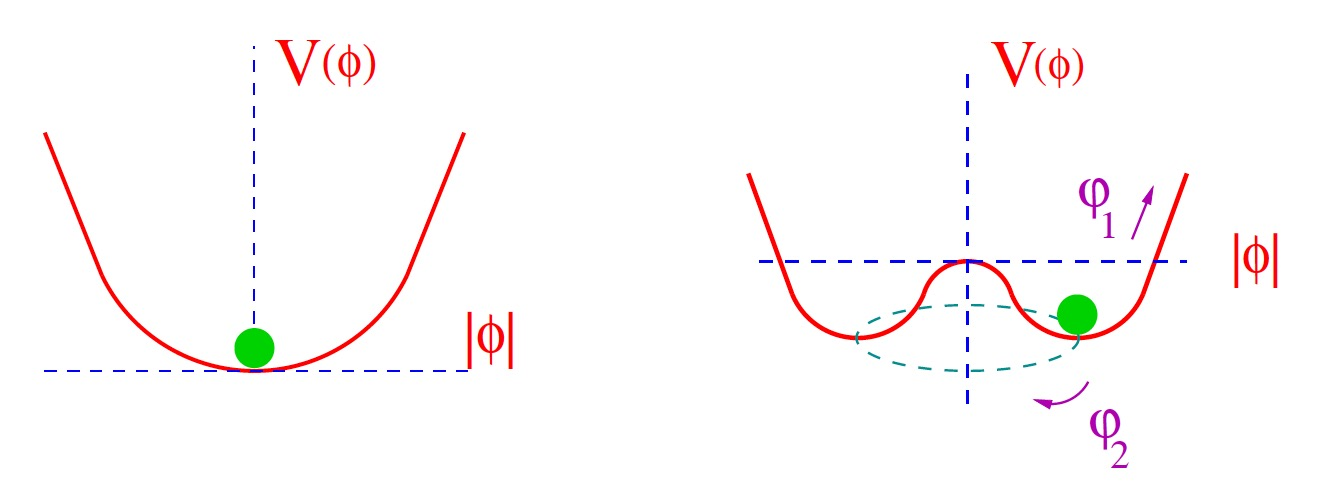
\includegraphics[width=0.85\textwidth]{figuresTHE/SSB.jpg}
  \end{center}
  \caption{
对称性自发破缺。
}
    \label{fig:SSB1}
\end{figure}


第一种可能$\mu^2>0$是仅具有单个基态的简单情形。
第二种情形$\mu^2<0$即对称性自发破缺,
过程中会出现一个无质量的粒子$\varphi_2$。
对称性自发破缺是物理系统的对称性自发破坏的过程,
它可以描述那些体系拉氏量的对称性和体系基态对称性不一致的物理系统。
无质量粒子的出现是一个与对称性自发破缺机制相关的一般性结果,
称为Goldstone定理:如果体系拉氏量在连续对称变换G作用下是不变的,
但是基态仅在G的子群H的作用下才具有不变性,
那么体系会存在与破缺的对称性相对应的多个无质量的Goldstone玻色子,
玻色子的个数等于G的生成元个数减去H的生成元个数。

\subsubsection{$W^{\pm}$和$Z$玻色子质量}
\label{sec:SSBWZ}
在第二种情况$\mu^2<0$下,对于拉氏量~\ref{eq:SSB1}~,当考虑一个$SU(2)$双重态的复标量场:
\begin{equation} 
\label{eq:SSB7}
\phi(x) \equiv 
 \left( \begin{array}{l} \phi^{(+)}(x) \\  \phi^{(0)}(x) \end{array} \right)
\end{equation}
类似电弱理论,利用规范原理构建一个在$SU(2)\otimes U(1)$局部规范变换下具有不变性的拉氏量$\mathcal{L}_S$:
\begin{equation} 
\label{eq:SSB8}
\begin{split}
& \mathcal{L}_S= (D_{\mu}\phi)^{\dagger}D_{\mu}\phi- \mu^2 \phi^{\dagger} \phi - h \left(  \phi^{\dagger} \phi   \right)^2 \quad (h>0, \mu^2<0)
%\end{equation}
%\begin{equation} 
%\label{eq:SSB9}
\\
&D^{\mu}\phi= \left[ \partial^{\mu}+ig\widetilde{W}^{\mu}(x)+ig'y_{\phi}B^{\mu}(x) \right] \psi_1(1), \quad y_{\phi}=\frac{1}{2}
\end{split}
\end{equation}
根据标量场$\phi(x)$与电磁场$A^{\mu}(x)$的耦合情况,即场$\phi^{(0)}(x)$不带电荷,场$\phi^{(+)}(x)$带有正电荷,
可以确定标量场的超荷$y_{\phi}$。
其中势能项与式~\ref{eq:SSB1}~类似,
体系具有无穷多个简并基态,满足:
\begin{equation} 
\label{eq:SSB10}
|\langle 0| \phi^{(0)} |0\rangle|=\sqrt{\frac{-\mu^2}{2h}}  \equiv \frac{v}{\sqrt{2}}
\end{equation}
因为电荷是守恒荷,只有中性标量场$\phi^{(0)}$才能获得真空期望值。
当体系处于某个特定的基态,
$SU(2)\otimes U(1)$规范对称性会自发的破缺到电磁相互作用的$U(1)$规范对称性,
根据Goldstone定理,会出现三个无质量的Goldstone玻色子。

当用四个实场$\theta^i(x)$和$H(x)$和基态来一般性的表示双重态的复标量场$\phi(x)$:
\begin{equation} 
\label{eq:SSB11}
\phi(x)=exp\left\{  i \frac{\sigma_i}{2}\theta^i(x)  \right\} \frac{1}{\sqrt{2}}
\left( \begin{array}{l} 0 \\  v+H(x) \end{array} \right)
\end{equation}
这样表示的目的是利用拉氏量的$SU(2)$局部规范对称性来消除对$\theta^i(x)$的依赖性,
%这样表示的目的在于拉氏量的$SU(2)$局部规范对称性可以消除对$\theta^i(x)$的依赖性,
这三个场就是与对称性自发破缺机制相关联的三个无质量的Goldstone玻色子场。
协变微分项~\ref{eq:SSB8}~中包含标量场和$SU(2)\otimes U(1)$规范玻色子的耦合,
当选取物理的规范,即单位规范令$\theta^i(x)=0$,并结合式~\ref{eq:EW15}~,标量场拉氏量~\ref{eq:SSB8}~的动能项可以化为:
\begin{equation} 
\label{eq:SSB12}
(D_{\mu}\phi)^{\dagger}D_{\mu}\phi \xrightarrow{\theta^i=0} \frac{1}{2} \partial_{\mu}H \partial^{\mu}H
+(v+H)^2\left\{    \frac{g^2}{4}W^{\dagger}_{\mu}W^{\mu} +\frac{g^2}{8\cos^2 \theta_W}Z_{\mu}Z^{\mu}    \right\}
\end{equation}
中性标量场$H(x)$为$W^{\pm}$和$Z$玻色子分别提供了一个二次项,即这三个规范玻色子有了质量:
\begin{equation} 
\label{eq:SSB13}
M_Z \cos \theta_W=M_W=\frac{1}{2}vg
\end{equation}
到此,可以看到对称性自发破缺机制怎样巧妙的为弱相互作用的中间玻色子$W^{\pm}$和$Z$赋予质量。
当要求拉氏量$\mathcal{L}_S$满足$SU(2)\otimes U(1)$局部规范对称,可以保证相应量子场论的可重整性,
引入对称性自发破缺机制之后,三个无质量的Goldstone玻色子会伴随着破缺的对称性而出现,
由于体系已有的规范对称性,可以通过选取单位规范将它们安全的从拉氏量中移除,
从而$W^{\pm}$和$Z$玻色子成功获得了质量。

\subsubsection{标量玻色子}
\label{sec:SSBH}

拉氏量~\ref{eq:SSB8}~中引入对称性自发破缺机制后,模型中出现了一个新的标量玻色子:希格斯玻色子$H$。
在单位规范下,拉氏量$\mathcal{L}_S$可以化简为如下形式:
\begin{equation} 
\label{eq:SSB14}
\mathcal{L}_S=\frac{1}{4}hv^4+\mathcal{L}_H+\mathcal{L}_{HG}
\end{equation}
其中:
\begin{equation} 
\label{eq:SSB15}
\mathcal{L}_H=\frac{1}{2}\partial_{\mu}H\partial^{\mu}H -\frac{1}{2}M_H^2 H^2
-\frac{M_H^2 }{2v}H^3 -\frac{M_H^2 }{8v^2}H^4
\end{equation}
\begin{equation} 
\label{eq:SSB16}
\mathcal{L}_{HG}= \left( 1+\frac{H}{v} \right)^2 M_W^2 W^{\dagger}_{\mu}W^{\mu} 
+ \frac{1}{2} \left( 1+\frac{H}{v} \right)^2 M_Z^2 Z_{\mu}Z^{\mu} 
\end{equation}
并且$H$玻色子具有质量:
\begin{equation} 
\label{eq:SSB17}
M_H=\sqrt{-2\mu^2}=\sqrt{2h}v
\end{equation}
式~\ref{eq:SSB16}~中希格斯玻色子的相互作用项有一个典型的特征:
它们总是与耦合在一起的玻色子的质量的平方成正比,由$M_H$,$M_W$,$M_Z$和真空期望值$v/\sqrt{2}$决定。


\subsubsection{费米子质量}
\label{sec:SSBF}

由于规范对称性的要求,费米子质量项:
\begin{equation} 
\label{eq:SSB18}
\mathcal{L}_F=-m\bar{\phi}\phi=-m(\bar{\phi}_L\phi_R+\bar{\phi}_R\phi_L)
\end{equation}
是不允许存在的。但是,由于在模型中已经引入了新的双重态复标量场,
于是可以构建如下规范对称的费米子-标量场耦合项,也称为Yukawa耦合:
\begin{equation} 
\label{eq:SSB19}
\begin{split}
\mathcal{L}_Y= & -c_1 (\bar{u},\bar{d})_L 
\left( \begin{array}{l} \phi^{(+)} \\  \phi^{(0)} \end{array} \right) d_R
-c_2 (\bar{u},\bar{d})_L 
\left( \begin{array}{l} \phi^{(0)\ast} \\  -\phi^{(-)} \end{array} \right) u_R
\\
& -c_3 (\bar{\nu}_e,\bar{e})_L 
\left( \begin{array}{l} \phi^{(+)} \\  \phi^{(0)} \end{array} \right) e_R
+ h.c.
\end{split}
\end{equation}
其中第二项涉及标量场的电荷共轭项$\phi^c \equiv i\sigma_2 \phi^*$,
引入对称性自发破缺并选取单位规范之后,
上述Yukawa耦合的拉氏量可以化简为:
\begin{equation} 
\label{eq:SSB20}
\mathcal{L}_Y=
-\frac{1}{\sqrt{2}}(v+H)\left(  c_1\bar{d}d+ c_2\bar{u}u +c_3\bar{e}e  \right)
\end{equation}
因此,费米子在对称性自发破缺机制下也获得了质量:
\begin{equation} 
\label{eq:SSB21}
m_d=c_1\frac{v}{\sqrt{2}}, \quad 
m_u=c_2\frac{v}{\sqrt{2}}, \quad 
m_e=c_3\frac{v}{\sqrt{2}}
\end{equation}
其中$c_i$为任意常数,用质量项表示拉氏量得:
\begin{equation} 
\label{eq:SSB22}
\mathcal{L}_Y=
-(1+\frac{H}{v})\left(  m_d\bar{d}d+ m_u\bar{u}u +m_e\bar{e}e  \right)
\end{equation}
可以看到轻子和夸克质量在标准模型中是自由参数,
而且费米子与希格斯玻色子之间的耦合强度与费米子质量成正比。
%但是其中未包含中微子质量项,因为实验上并未观测到希格斯玻色子与中微子有明显耦合的现象。


\section{希格斯玻色子}
\label{sec:Higgs}

对称性自发破缺机制中的关键标量玻色子,希格斯玻色子的寻找已经在粒子物理领域持续了数十年。
理论提出来之后二十多年,
CERN的大型正负电子对撞机和Tevatron的正负强子对撞机先后对希格斯玻色子质量的给出严格的区间限制~\cite{TEVN,LEP},
在2010年,LHC以比之前更高的质心能量和总积分亮度开始取数,将会在第~\ref{cha:EXP}~章介绍LHC,
最后在2012年,LHC上的两个大型探测器ATLAS和CMS(The Compact Muon Solenoid)终于发现了一个与标准模型中希格斯玻色子相符合的粒子~\cite{ATLASHIGGS,CMSHIGGS},
其质量在大约125GeV左右,
这是粒子物理学史上一个重大的里程碑。
在发现希格斯玻色子之后,接下来实验上非常重要的一个任务便是
对希格斯玻色子的性质进行精确测量,包括自旋、宇称、耦合和产生机制等,
这些都是对标准模型必不可少的检验。

\subsection{希格斯玻色子的产生}
\label{sec:HiggsPD}

标准模型中希格斯玻色子主要有以下几种产生模式~\cite{HANDHIGGS}:
图示~\ref{fig:ggF}~胶子融合(Gluon–gluon fusion, ggF);
图示~\ref{fig:VBF}~矢量玻色子融合(Vector-boson fusion, VBF);
图示~\ref{fig:WZH}~矢量玻色子联合产生道(WH+ZH, VH);
图示~\ref{fig:ttH}~t夸克联合产生道($tH+t\bar{t}H$)。

\begin{figure}
  \begin{center}
    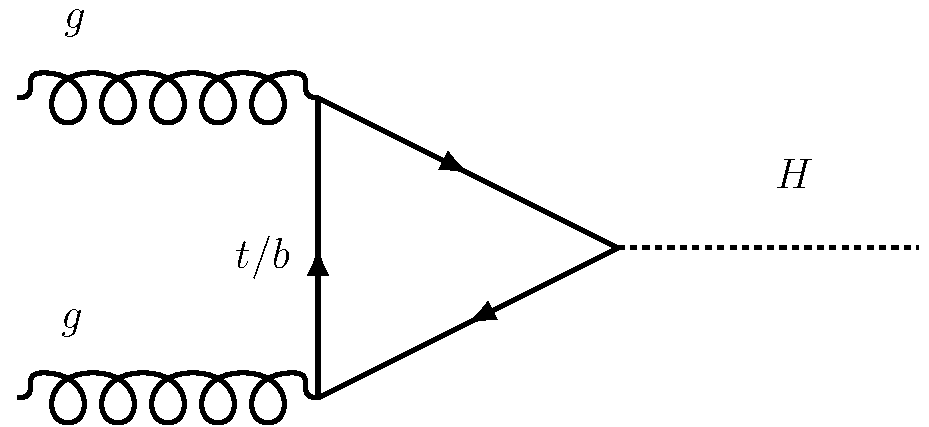
\includegraphics[width=0.5\textwidth]{figuresTHE/ggF.pdf}
  \end{center}
  \caption{
希格斯玻色子产生模型:领头阶胶子融合产生模式。
}
    \label{fig:ggF}
\end{figure}

\begin{figure}
  \begin{center}
    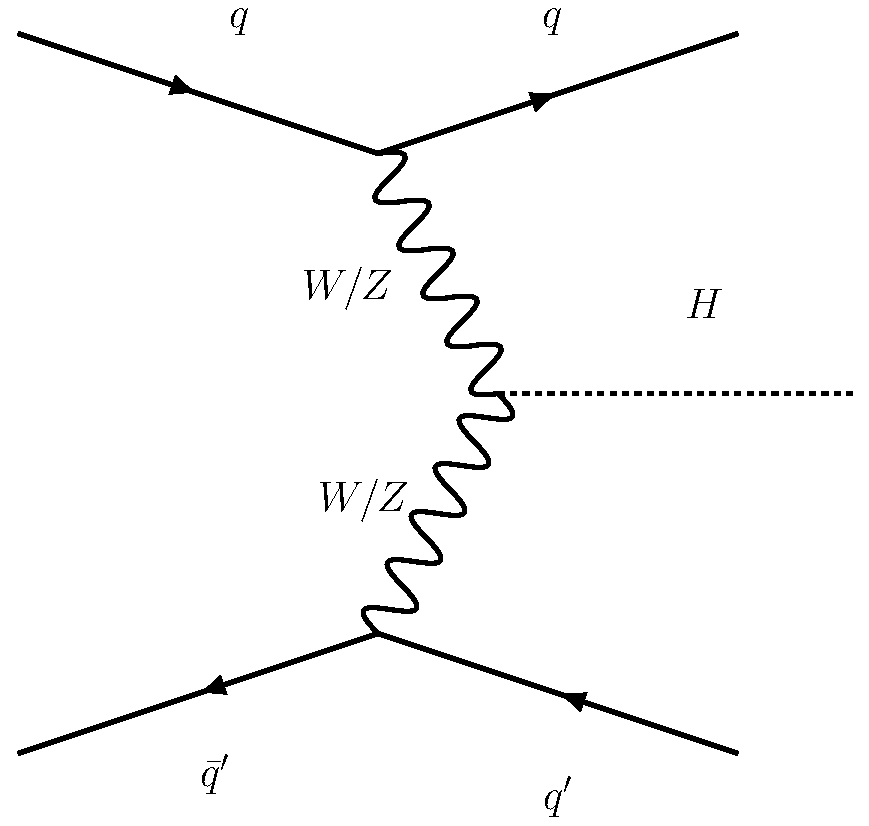
\includegraphics[width=0.5\textwidth]{figuresTHE/VBF.pdf}
  \end{center}
  \caption{
希格斯玻色子产生模式:领头阶矢量玻色子融合。
}
    \label{fig:VBF}
\end{figure}


\begin{figure}
  \begin{center}
    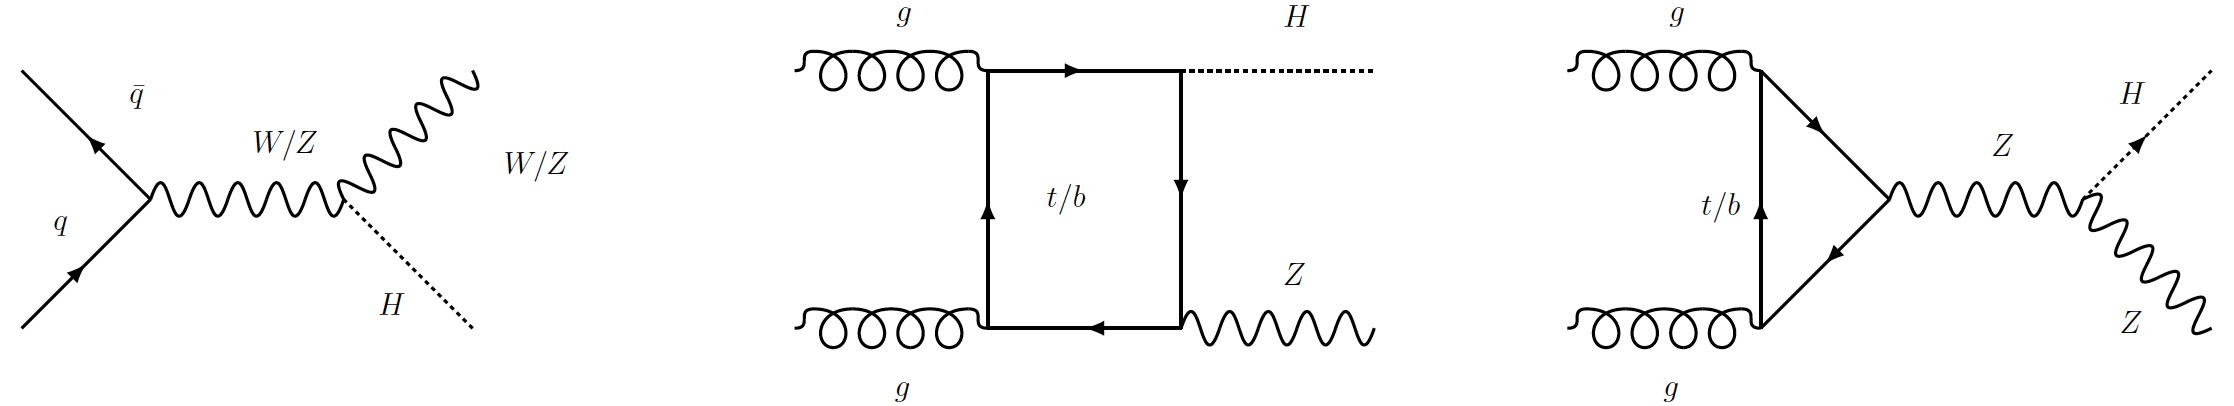
\includegraphics[width=0.98\textwidth]{figuresTHE/WZH.jpg}
  \end{center}
  \caption{
希格斯玻色子产生模型:领头阶矢量玻色子联合产生道。
}
    \label{fig:WZH}
\end{figure}

\begin{figure}
  \begin{center}
    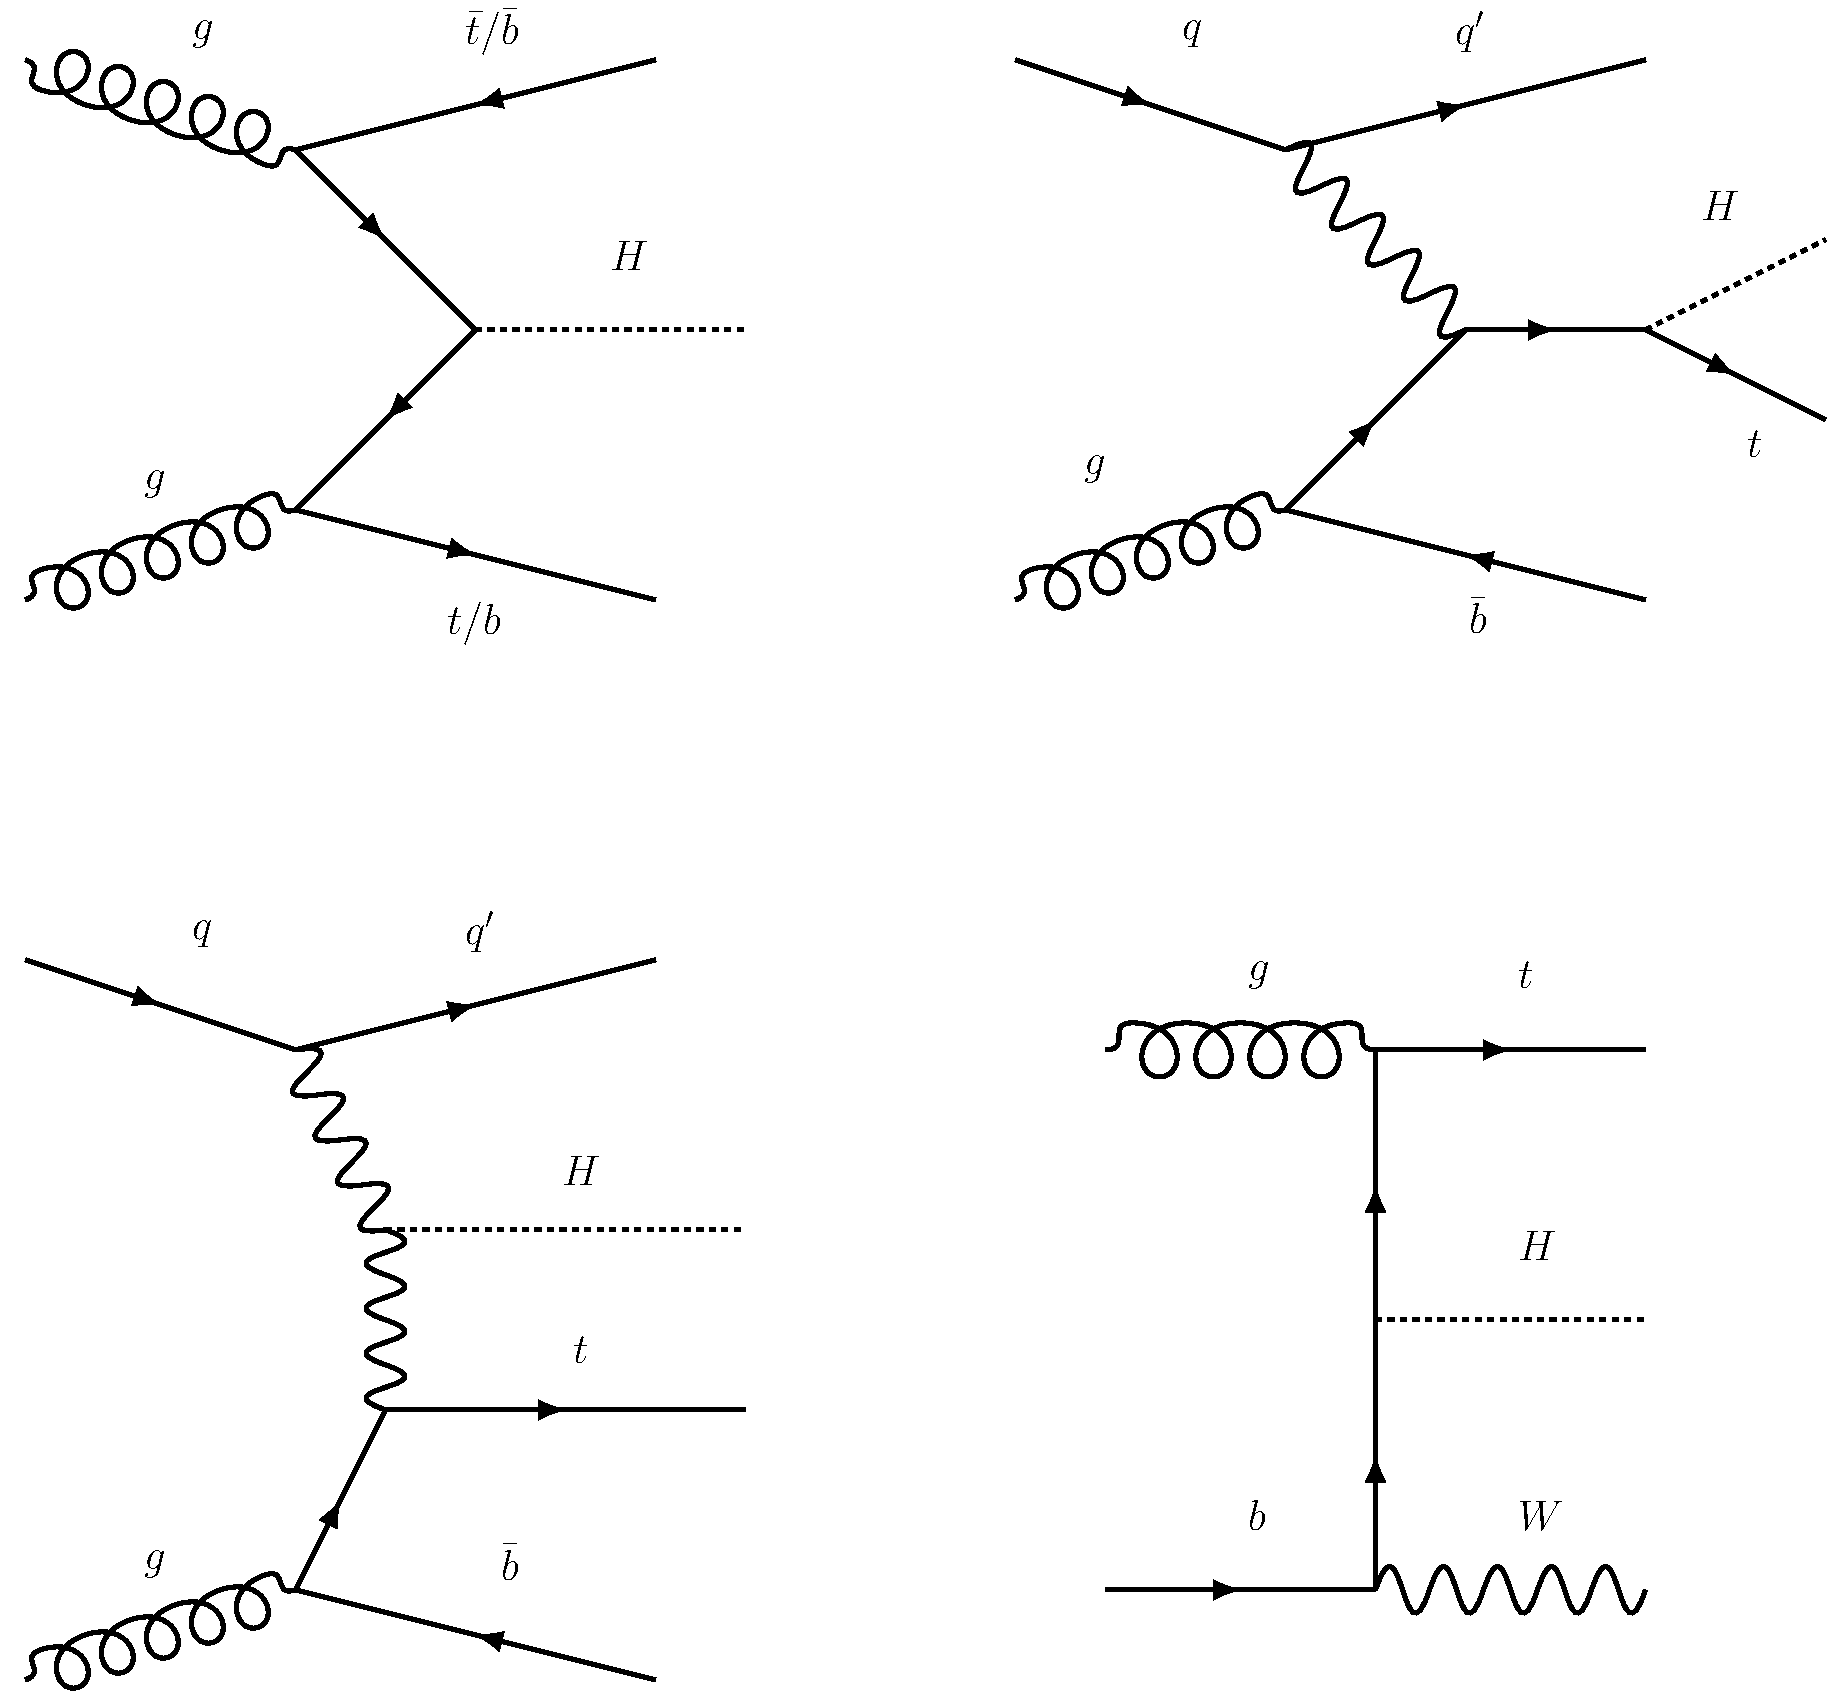
\includegraphics[width=0.85\textwidth]{figuresTHE/ttH.pdf}
  \end{center}
  \caption{
希格斯玻色子产生模式:领头阶矢t夸克联合产生道。
}
    \label{fig:ttH}
\end{figure}

各个产生模式的截面的大小取决于希格斯玻色子质量、碰撞强子的类型和质心系能量。
结合$Run\_1$计划期间ATLAS和CMS所收集的所有数据,测得希格斯玻色子的质量为$m_H=125.09\pm 0.21(stat.)\pm 0.11(syst.)GeV$~\cite{HIGGSMASS}。
图~\ref{fig:SM23}~中左图给出了LHC上质子-质子对撞的质心系能量固定为$\sqrt{s}=13TeV$时,不同产生模式的截面随着希格斯玻色子质量的变化关系,
而右图展示了在希格斯玻色子质量为$M_H=125GeV$情况下,不同产生模式的截面随着质心系能量的变化关系。


\begin{figure}  
  \begin{center}
    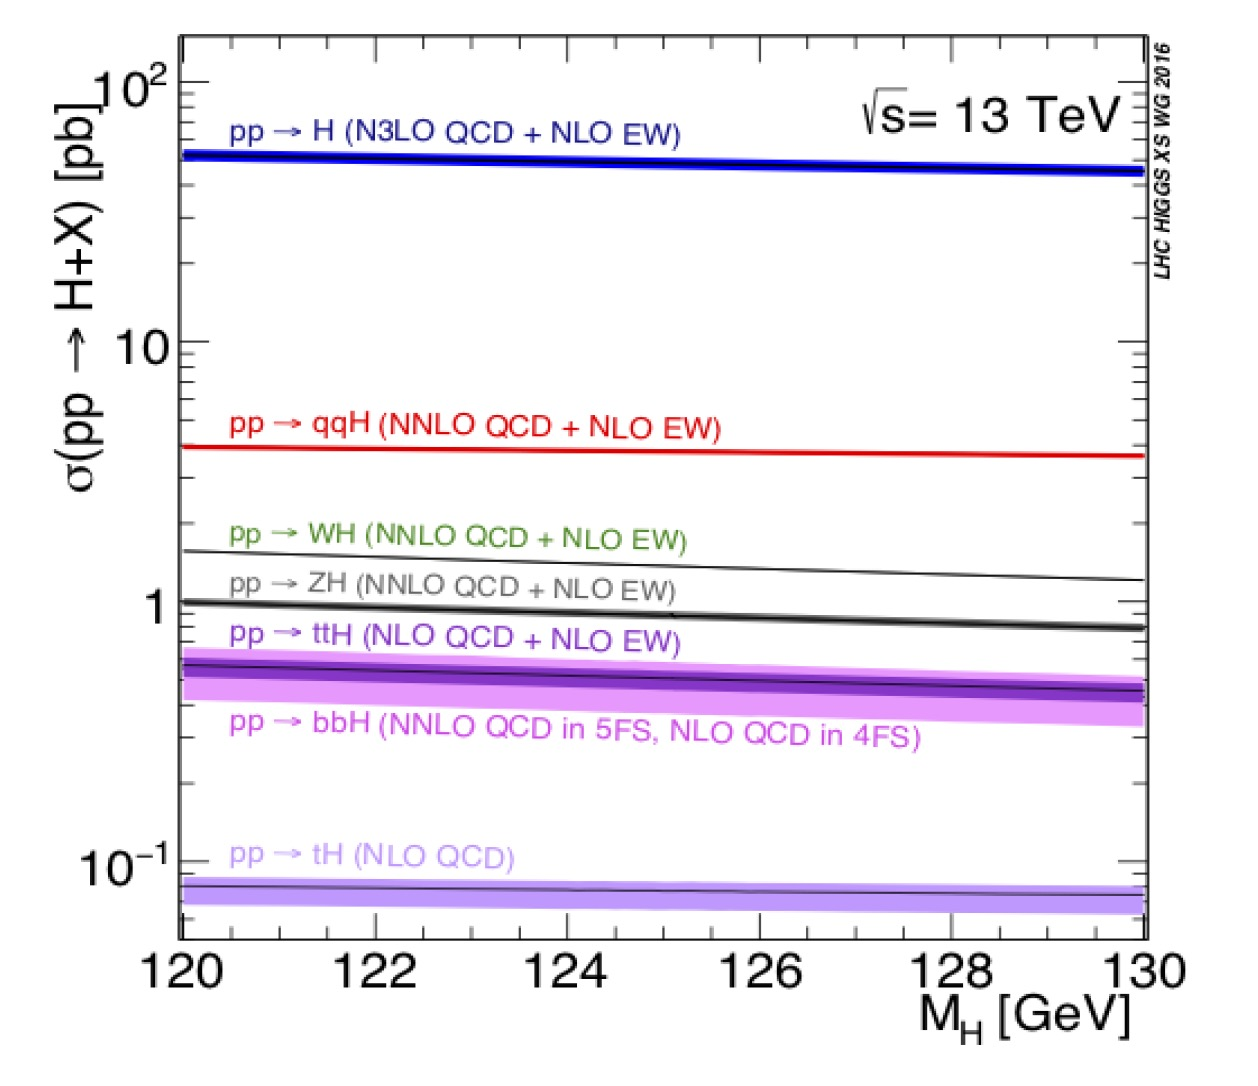
\includegraphics[width=0.49\textwidth]{figuresTHE/SM2.jpg}
    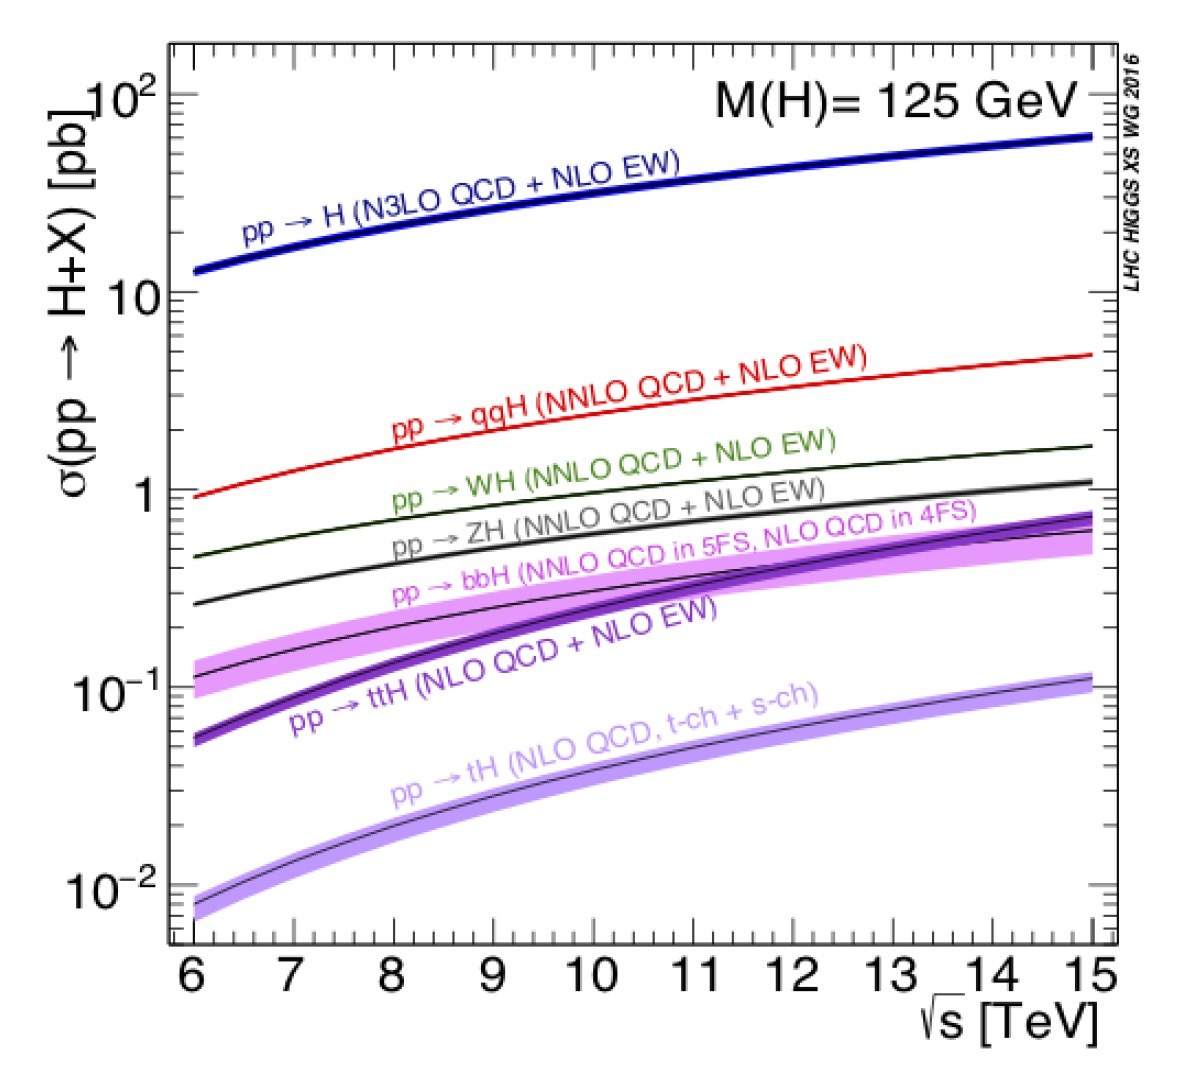
\includegraphics[width=0.49\textwidth]{figuresTHE/SM3.jpg}
  \end{center}
  \caption{
  LHC上质子-质子对撞的质心系能量固定为$\sqrt{s}=13TeV$时,不同产生模式的截面随着希格斯玻色子质量的变化关系(左图),
以及希格斯玻色子质量为$M_H=125GeV$时,不同产生模式的截面随着质心系能量的变化关系(右图)。
    }
  \label{fig:SM23}
\end{figure}



\subsection{希格斯玻色子的衰变}
\label{sec:HiggsDC}

为了表征不同衰变模式的相对强度,引入
衰变分支比(Branching ratio, BR),
它是指相对于衰变粒子的总数,
以单独的衰变模式f进行衰变的粒子所占的分数,
它与部分衰变宽度和总衰变宽度$\Gamma$有关:
\begin{equation} 
\label{eq:HiggsDC1}
BR(H \rightarrow f)= \frac{\Gamma(H \rightarrow f)}{\sum_f \Gamma(H \rightarrow f)}
\end{equation}
如图~\ref{fig:SM45}~所示,是标准模型预言的希格斯玻色子不同模式的衰变分支比与希格斯玻色子质量的关系~\cite{HANDHIGGS},
左图所示质量区间为80到120GeV,右图是120到130GeV。

\begin{figure}  
  \begin{center}
    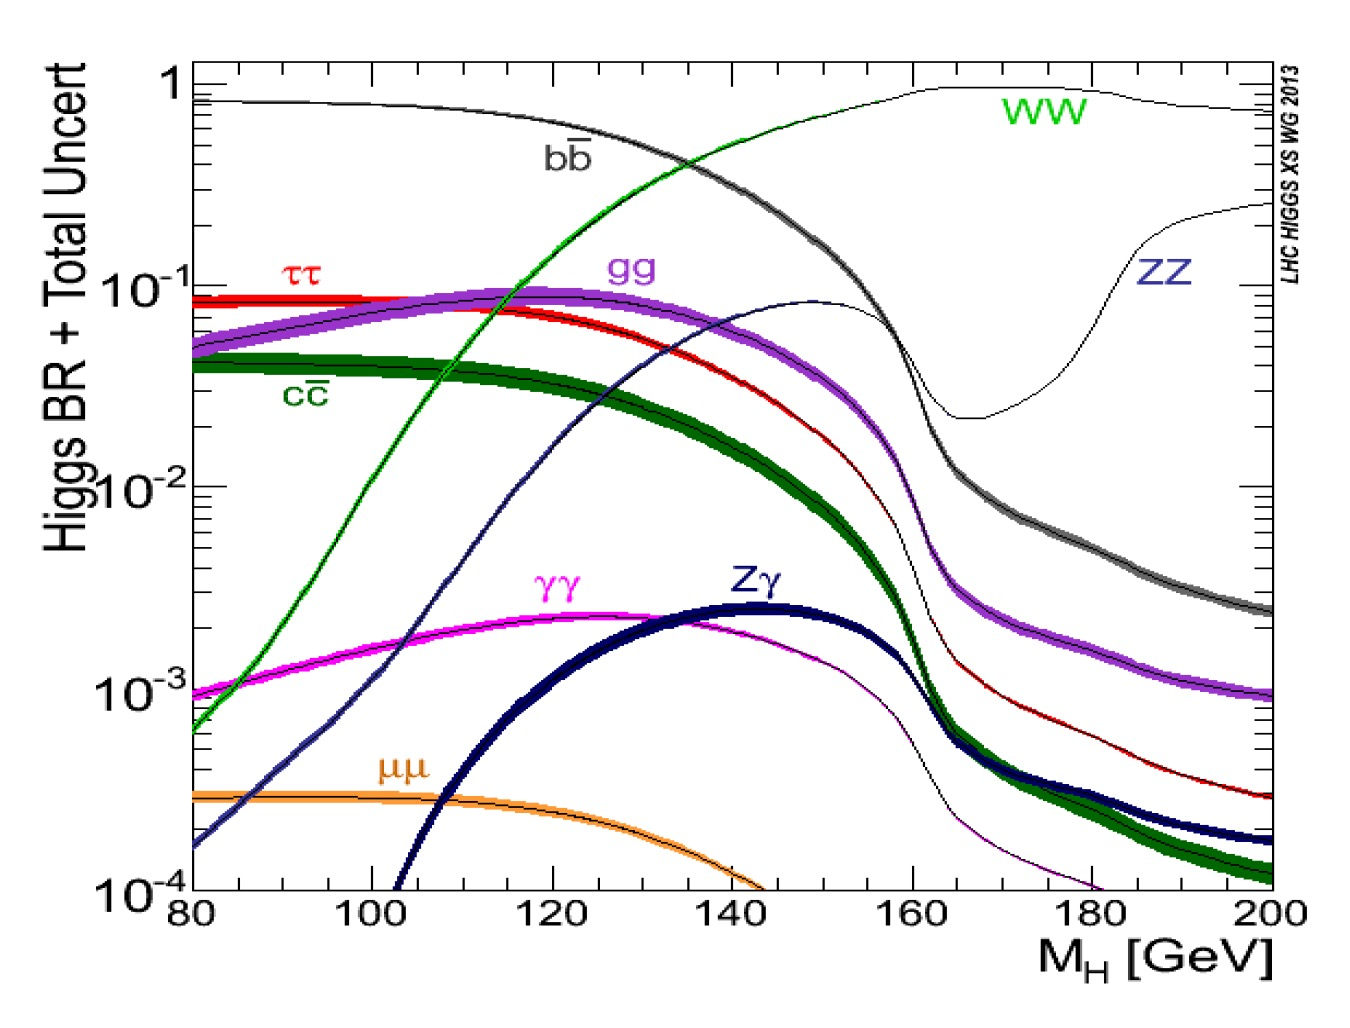
\includegraphics[width=0.49\textwidth]{figuresTHE/SM4.jpg}
    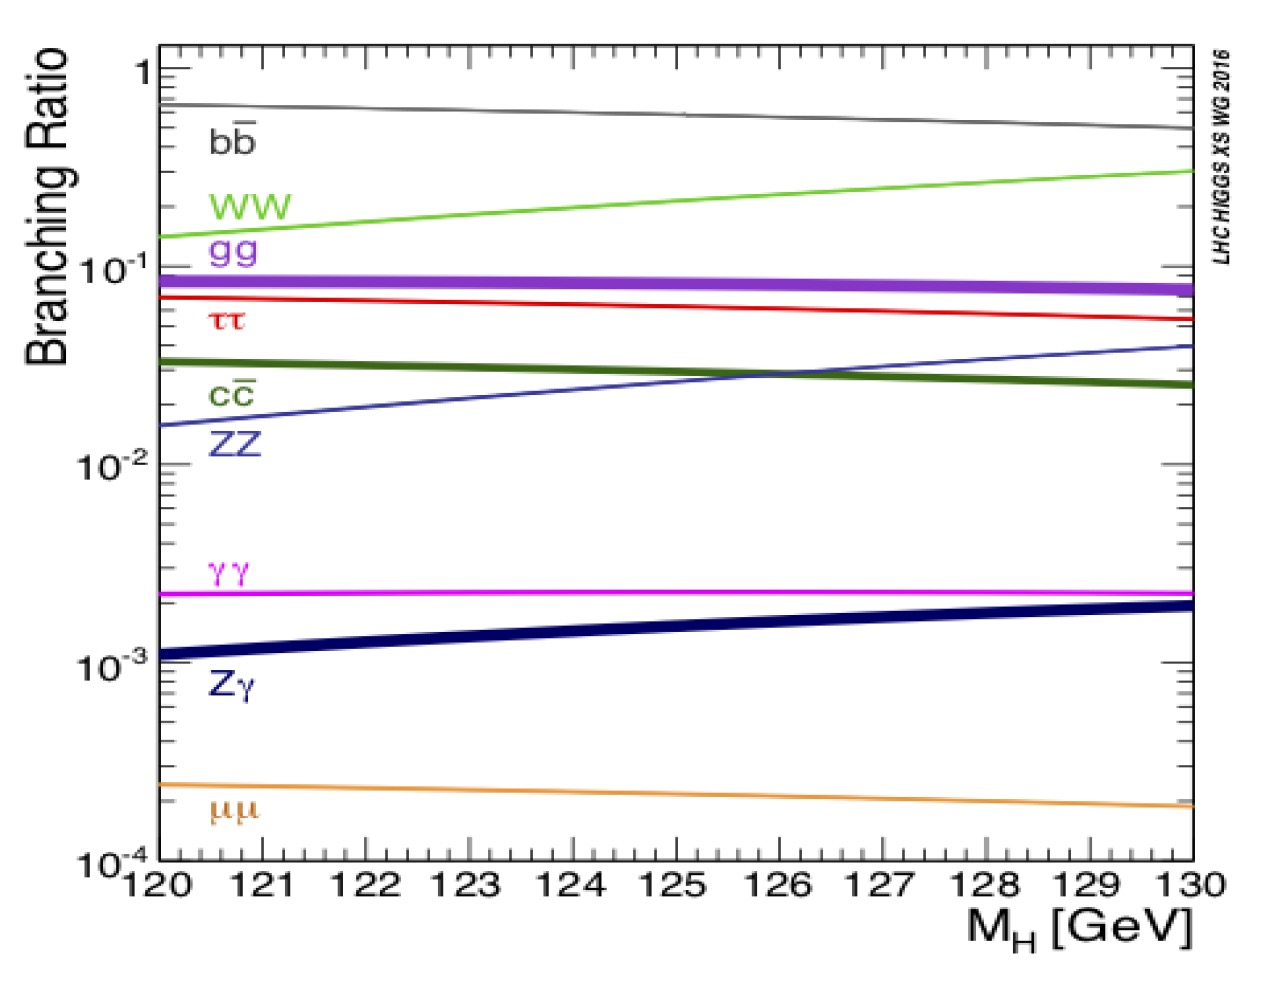
\includegraphics[width=0.49\textwidth]{figuresTHE/SM5.jpg}
  \end{center}
  \caption{
希格斯玻色子不同模式的衰变分支比与希格斯玻色子质量的关系。左图所示质量区间为80到120GeV,右图是120到130GeV。
    }
  \label{fig:SM45}
\end{figure}

表~\ref{tab:SMTab1}~列出了当希格斯玻色子质量取$M_H=125GeV$时,各个可能衰变模式的衰变分支比。
如前面所指出的,由于费米子与希格斯玻色子的耦合强度与费米子质量成正比,
因此在末态为费米子的衰变模式中,希格斯玻色子更加倾向于衰变成质量较大的费米子。

\begin{table}[htbp]
      \caption{在希格斯玻色子质量为$m_H=125GeV$时,标准模型中希格斯玻色子各个衰变模式的衰变分支比。}
      \label{tab:SMTab1}
      \centering
      
%      \begin{tabular}{|c|c|c|c|c|c|c|c|c|}
 %       \hline
 %        Decay channel~$(H \rightarrow )$ & $b \bar{b}$ & $W^+W^-$ & $gg$ & $\tau^+\tau^-$ & $ZZ$ & $\gamma\gamma$ & $Z\gamma $& $\mu^+\mu^-$ \\
 %       \hline
 %        Branching ratio & $5.81\times 10^{-1}$ & $2.15\times 10^{-1}$ & $8.18\times 10^{-2}$ & $6.26\times 10^{-2}$ & $2.64\times 10^{-2}$ & $2.27\times 10^{-3}$ & $1.54\times 10^{-3}$ & $2.17\times 10^{-4}$   \\
 %       \hline
 %    \end{tabular}
      \begin{tabular}{|c|c|}
      \hline
      Decay channel~$(H \rightarrow )$ & Branching ratio \\
       \hline
        $b \bar{b}$ & $5.81\times 10^{-1}$   \\
         \hline
        $W^+W^-$ &  $2.15\times 10^{-1}$ \\
         \hline
        $gg$  &  $8.18\times 10^{-2}$  \\
         \hline
        $\tau^+\tau^-$  &  $6.26\times 10^{-2}$  \\
         \hline
        $ZZ$  & $2.64\times 10^{-2}$  \\
         \hline
        $\gamma\gamma$  & $2.27\times 10^{-3}$   \\
         \hline
        $Z\gamma $ & $1.54\times 10^{-3}$  \\
         \hline
        $\mu^+\mu^-$ & $2.17\times 10^{-4}$  \\
        \hline 
      \end{tabular}
\end{table}


\subsection{高横动量希格斯玻色子衰变到双b夸克的标定动机}
\label{sec:BoostedHiggs}

%而对于所测定的质量,标准模型预测的衰变分支比最大的模式是$H\rightarrow b \bar{b}$,达到了$58\%$,
%但也由于QCD和t夸克本底比较大,使得该衰变模式的鉴定非常困难。
%在这个背景下,第~\ref{cha:Xbb}~章介绍了一种基于机器学习的标定算法,
%用于标定高横动量的$H\rightarrow b \bar{b}$,
%它不仅实现了质量去关联,而且还能保持非常出色的本底排除率。
%其中,尽管$H\rightarrow b\bar{b}$衰变道是希格斯玻色子的主要衰变模式,占高达$58\%$的分支比,

对于实验测定的希格斯质量,
从表~\ref{tab:SMTab1}~中可以看到$H\rightarrow b\bar{b}$衰变道是希格斯玻色子的主要衰变模式,
所占分支比高达$58\%$,
但也由于来自QCD过程和t夸克衰变的本底非常大,使得在LHC上面观测这个衰变模式变得很困难。
通过要求事例中包含孤立的轻子,可以显著的降低QCD本底,因此寻找$H\rightarrow b\bar{b}$衰变道灵敏度最高的产生模式是VH,
在2018年,ATLAS合作组和CMS合作组分别利用$79.8fb^{-1}$和$41.3fb^{-1}$的数据通过VH产生模式观测到显著的$H\rightarrow b\bar{b}$事例,
显著性分别达到了4.9和4.8倍的标准差~\cite{AHbb8,CHbb3},
随后在2020年,ATLAS合作组利用$139fb^{-1}$的数据观测到了更加丰富的$H\rightarrow b\bar{b}$事例~\cite{AHbb5}。
但是也有一部分研究通过其他产生模式来测定$H\rightarrow b\bar{b}$衰变道,
比如$t\bar{t}H$~\cite{AHbb7,AHbb8,CHbb1}、VBF~\cite{AHbb6}和高横动量区的ggF~\cite{CHbb3}。

而高横动量的$H\rightarrow b\bar{b}$衰变与低横动量的$H\rightarrow b\bar{b}$衰变的拓扑性质不一样,
如图~\ref{fig:Boosted1}~所示,在探测器中,来自高横动量希格斯玻色子衰变的两个b夸克接近准直,
会合并到一个大的喷注即LR-jet当中,将会在第~\ref{sec:JET}~小节介绍LR-jet的概念,
通过其整体性可以更加容易的鉴定$H\rightarrow b\bar{b}$事例。
%依靠其整体性使得$H\rightarrow b\bar{b}$事例更容易鉴定。
而且在许多超出标准模型的新物理模型中~\cite{BSMHIGGS1,BSMHIGGS2,BSMHIGGS3}都引入了能与标准模型中希格斯玻色子耦合的新粒子的存在,
这些新粒子的质量都很大,衰变产生的希格斯玻色子将会具有很高的横动量。
因此对高横动量的$H\rightarrow b\bar{b}$衰变的
%研究或者
标定对希格斯玻色子性质的精确测量和新物理的寻找都有着重要意义。
这篇论文第~\ref{cha:Xbb}~章中便介绍了一种基于机器学习的标定算法,用于标定高横动量$H\rightarrow b \bar{b}$衰变。


\begin{figure}
  \begin{center}
    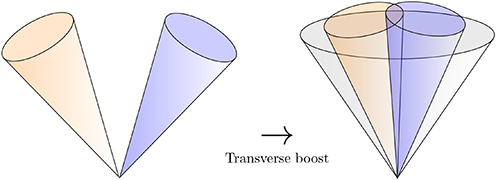
\includegraphics[width=0.75\textwidth]{figuresXbb/Boosted.jpg}
  \end{center}
  \caption{
来自高横动量希格斯玻色子衰变的两个b夸克接近准直,从而合并到一个LR-jet当中。
  }
    \label{fig:Boosted1}
\end{figure}







\section{超出标准模型的新物理}
\label{sec:BSM}

在标准模型建立的过程中,
实验上不断的以极高的精度验证了其正确性,
%其不断的以极高的准确性得到了验证,
并且在理论预测和实验观测之间也保持着高度的一致。
但是,仍然存在一部分标准模型不能解释的现象。

标准模型未能解释暗物质~\cite{DARKMATTER1}从何而来,也没有提供暗物质的候选粒子。
在1930年,F. Zwicky观测到后发星系团(Coma cluster)中星系的速度弥散(Velocity dispersion)约为1000$km~s^{-1}$,
这比根据实际发光物质所估计的速度弥散80$km~s^{-1}$要大的多,
这表明存在“看不见”的物质即暗物质为星系团提供额外的吸引力将星系保持在星系团内部~\cite{DARKMATTER2}。
在那以后,有更多的实验证据为暗物质提供了有力的支持~\cite{DARKMATTER1},
根据宇宙学观测的结果,暗物质贡献了宇宙总物质的$27\%$,
而标准模型所描述的基本粒子仅占$5\%$。

标准模型中未包含引力。引力作为一种基本的相互作用,可以由广义相对论~\cite{GRE}来描述,
标准模型虽然统一了强、弱和电磁相互作用,但是它不能在量子场论的框架下诠释引力的规范理论。
其中重要的原因是,标准模型中引入引力子之后将不具有可重整性~\cite{GRE1},
而且电弱相互作用和引力相互作用之间存在层级问题(The hierarchy problem)~\cite{HP},
电弱对称破缺的能标($\sim 10^{2}GeV$)比引力的基础能标即普朗克能标($\sim 10^{19}GeV$)小多个数量级。

还有诸如Yukawa耦合常数的层级问题、中微子质量起源和宇宙中正反物质不对称等问题。
都表明了标准模型本身并不是完整的,不能作为物质世界的终极理论。



\subsection{在双喷注末态的不变质量谱中寻找新物理的动机}
\label{sec:BSMDijet}

为了解决这些问题,理论物理学家发展了许多超出标准模型的新物理理论(Physics beyond the Standard Model, BSM)。
其中的一部分新物理模型~\cite{qstar1,qstar2,zprime1,zprime3,wprime1,Chizhov:2009fc,Chizhov:2010jg,DM1,DM2,DM3,qbh1,qbh2,RS1,RS2,ADD}
预言了能与标准模型中夸克或者胶子耦合的新的重粒子的存在,
这些新粒子如果存在的话能通过高能质子-质子对撞产生,并衰变成两个能量很高的夸克或者胶子,
以两个喷注即jet的形式被探测器探测到,将会在第~\ref{sec:JET}~小节介绍jet的概念,
图~\ref{fig:BSMDijet1}~为该过程所对应的费曼图~\cite{FEYNR}。
在标准模型中,双喷注末态事例主要来自于QCD过程,
而QCD预言的双喷注末态的不变质量谱$m_{jj}
$\footnote{自然单位制下,两个物理对象的不变质量定义为$m_{12}=\sqrt{(E_1+E_2)^2-(\vec{p_1}+\vec{p_2})^2}$,其中($E_1$,$\vec{p_1}$)、($E_2$,$\vec{p_2}$)分别为两个物理对象的能量和动量。}
是平滑下降的,
若是有一个非标准模型的新粒子衰变到两个夸克或者胶子,在QCD预言的平滑下降的$m_{jj}$上便会出现一个共振峰,
对应于新粒子的质量,可以通过这个手段来寻找新物理~\cite{UA3}。
这篇论文第~\ref{cha:Dijet}~章介绍的物理分析便是通过在双喷注末态的不变质量谱上搜索局部突出的共振峰,在TeV量级的高质量区间寻找超出标准模型的新粒子。
这里选取了其中一部分新物理模型作为基准模型来优化分析,同时用来评估同类型分析的进展。

\begin{figure}
  \begin{center}
    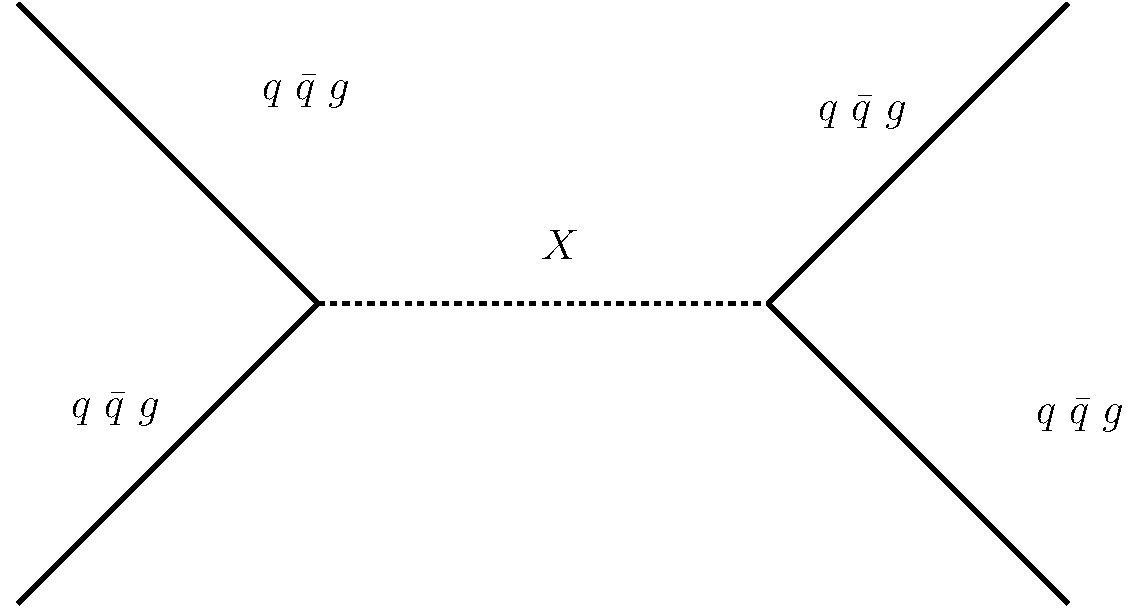
\includegraphics[width=0.5\textwidth]{figuresTHE/SChl.pdf}
  \end{center}
  \caption{
新粒子的产生模式。其中X表示新粒子。
}
    \label{fig:BSMDijet1}
\end{figure}


%为了解决这些问题,理论物理学家发展了许多超出标准模型的新物理理论(Physics beyond the Standard Model, BSM)。
%如图~\ref{fig:SChl}~所示,第~\ref{cha:Dijet}~章中的分析旨在通过新物理共振态的s道产生模式来寻找超出标准模型的新物理~\cite{FEYNR},
%并选取了一些新物理模型作为基准模型来优化分析,同时用来评估同类型分析的进展。
%这里将简要介绍这些所选的基准理论模型和它们背后的动机。


%\begin{figure}
 % \begin{center}
   % 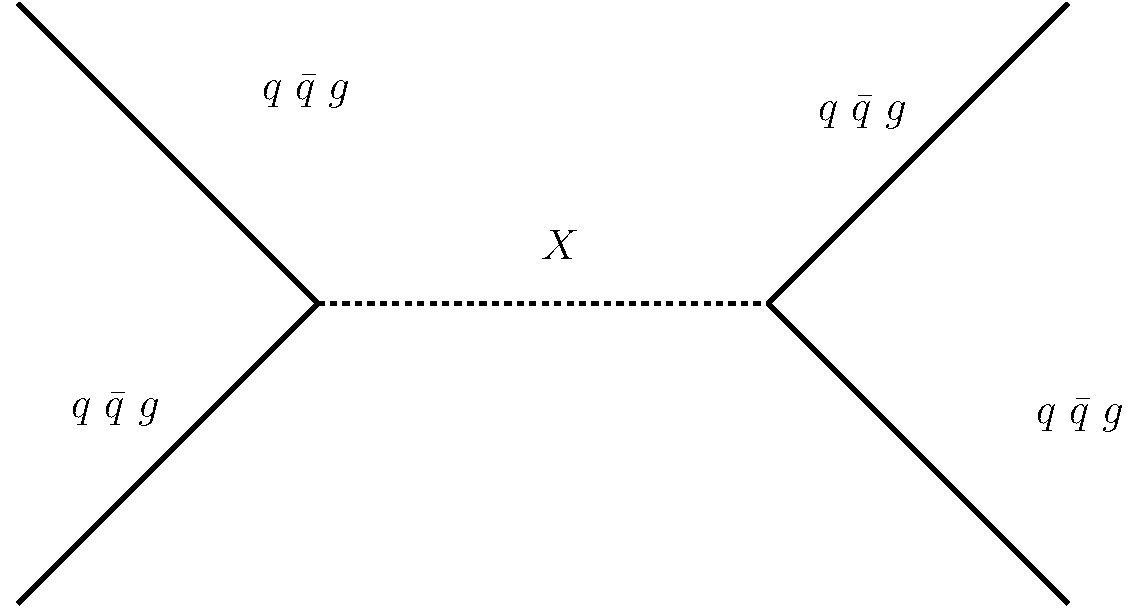
\includegraphics[width=0.5\textwidth]{figuresTHE/SChl.pdf}
  %\end{center}
  %\caption{
%新物理共振态的s道产生模式。
%}
  %  \label{fig:SChl}
%\end{figure}


\subsection{暗物质$Z'$模型}
\label{sec:ZPrime}

暗物质$Z'$模型~\cite{DM1,DM2,DM3}是将标准模型中的基本粒子与暗物质(Dark Matter, DM)媒介子$Z'$和暗物质候选粒子$\chi$联系起来的一个模型,
其中暗物质媒介子$Z'$是一个来自额外$U(1)$规范群的轴矢量玻色子,
如图~\ref{fig:ZChl}~所示,它能与暗物质费米子$\chi$耦合,也可以与标准模型中夸克耦合,
对应的拉氏量为:
\begin{equation} 
\label{eq:ZPrime1}
\mathcal{L}_{axial-vector}=g_{\chi} Z'_{\mu} \bar{\chi} \gamma^{\mu} \gamma^5 \chi +
g_{SM} \sum_{q=u,d,s,c,b,t} \left( Z'_{\mu} \bar{q} \gamma^{\mu} \gamma^5 q \right)
\end{equation}
其中$g_{SM}$是
%暗物质媒介子
DM $Z'$与标准模型中夸克的耦合常数,
$g_{\chi}$是DM $Z'$与
%暗物质费米子
$\chi$之间的耦合常数,
DM $Z'$和$g_{\chi}$的质量也是模型中的未知参数。
通过DM $Z'$与夸克之间的耦合可以在探测器上寻找$Z'$。

\begin{figure}
  \begin{center}
    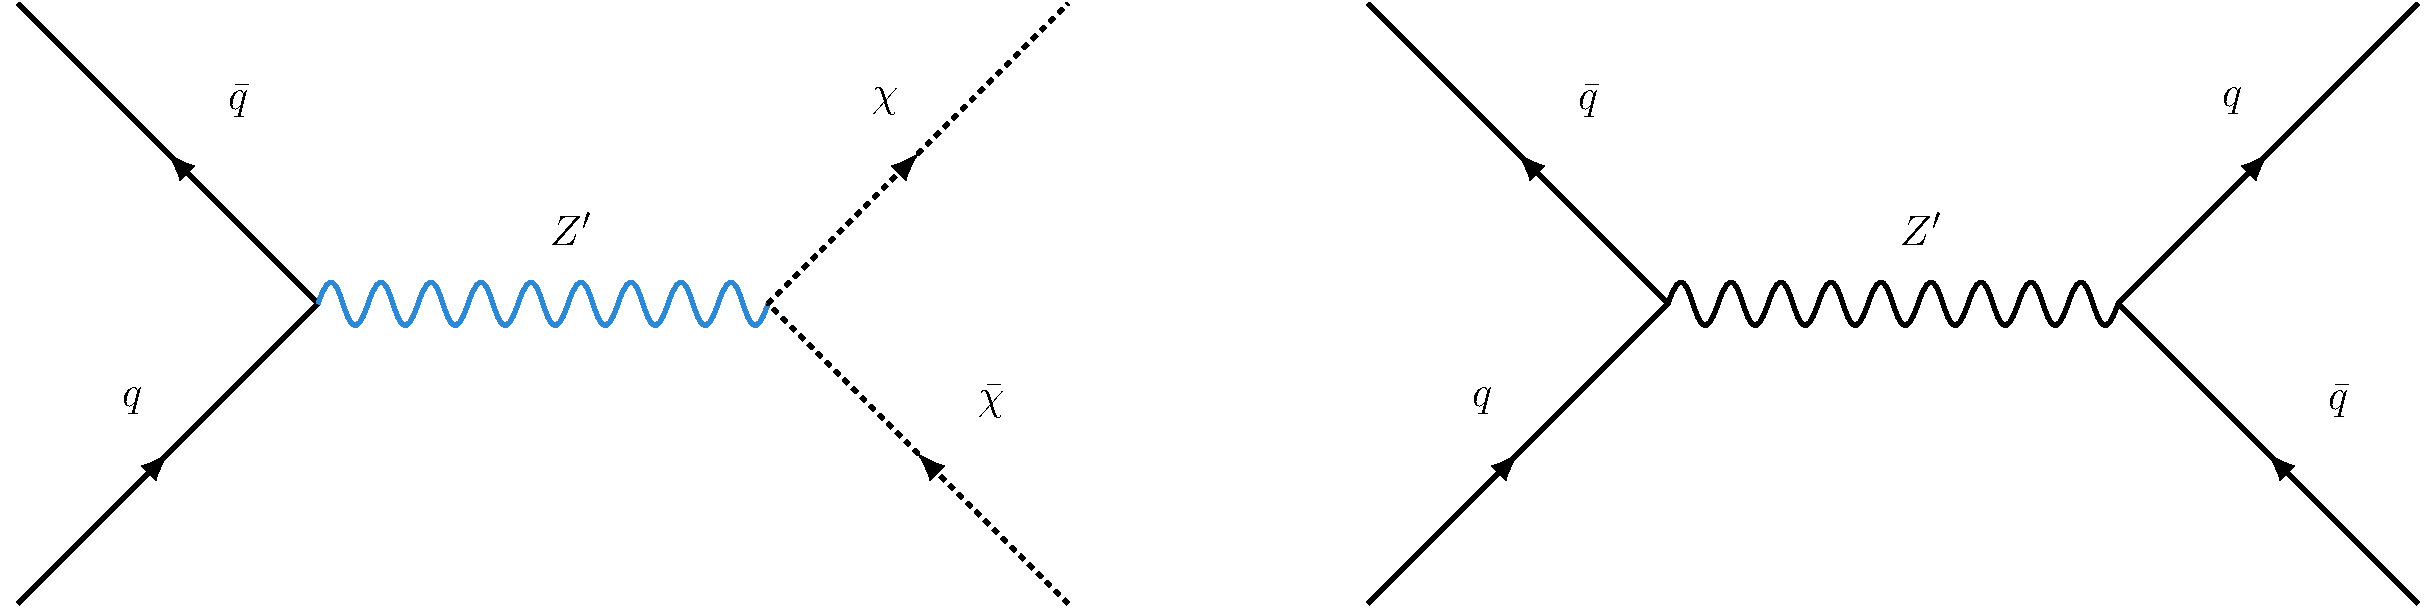
\includegraphics[width=0.9\textwidth]{figuresTHE/ZChl.pdf}
  \end{center}
  \caption{
暗物质媒介子$Z'$的两种衰变模式。左图$Z'\rightarrow \chi+\bar{\chi}$。右图$Z'\rightarrow q+\bar{q}$。
}
    \label{fig:ZChl}
\end{figure}

\subsection{Kaluza-Klein引力子和量子黑洞}
\label{sec:KKG}
作用力之间的层级问题使得引力比其他相互作用弱很多。
可能的一个解释是,引力本来与其他相互作用有着比较接近的强度,
但是因为它可以在更高维的时空中传播,在可观测的四维时空中就表现很弱。
基于这种猜想,有两种主流的额外维理论模型:Randall-Sundrum模型~\cite{RS1,RS2}和
Arkani-Hamed Dimopoulos Dvali模型~\cite{ADD}。
模型中高维时空的引入可以将引力的基础能标(The fundamental scale of gravity)降低到TeV的量级,
相应
Randall-Sundrum模型中
的Kaluza-Klein(KK)引力子(Graviton, G)便可以在LHC上产生并衰变成两个夸克或者胶子,
同时
Arkani-Hamed Dimopoulos Dvali模型中
质量在TeV量级的量子黑洞~\cite{qbh1,qbh2}也可以在LHC上形成并衰变成两个夸克或者胶子,
在一定的质量范围内被探测器探测到。

%\subsection{量子黑洞}
%\label{sec:QBH}
%上述高维时空引入之后,在降低引力能标的同时,
%LHC上高能质子-质子对撞也可能形成质量在TeV量级量子黑洞~\cite{qbh1,qbh2},
%并且能衰变到夸克或者胶子。


\subsection{重规范玻色子}
\label{sec:WZPrime}
在许多BSM理论中,都引入了额外的规范对称性,
从而会出现新的规范玻色子。
这里考虑了连续标准模型(The Sequential Standard Model, SSM)~\cite{zprime1,zprime3,wprime1}中
质量比较大的两种规范玻色子$W'$和$Z'$,
它们的质量也在TeV尺度,能衰变到两个夸克。

\subsection{激发态夸克}
\label{sec:QStar}
激发态夸克$q^*$($q=(u,d,c,s,b)$)~\cite{qstar1,qstar2}来自于一种复合夸克模型,模型中$q^*$的不是基本粒子,
而是具有内部结构的束缚态,能衰变到一个夸克和一个胶子。
模型的出发点是为了解释夸克质量的层级结构和三代问题。

\subsection{手征激发态玻色子$W^*$}
\label{sec:WStar}

手征激发态玻色子$W^*$~\cite{Chizhov:2009fc,Chizhov:2010jg}来自于一个拓展模型,
其将标准模型中弱相互作用的规范群$SU(2)$扩展成$SU(3)$,
相应的对称性自发破缺的能标在TeV量级。
%并通过TeV能标的对称性自发破缺。
%模型中会出现一个相应的带电矢量玻色子$W^*$,它能与标准模型中的费米子耦合。





















